%% I have improved the format a bit (but you need to add page breaks before chapters). You have written it in the first person, which is not good for this level of dissertation. Can you get rid of that .. and say something like "This dissertation" ...

%% Search for every occurrence of "I" and change it to something like "The dissertation...". Only in the personal reflection part to you write in the first person.
%% Make sure you talk about this dissertation being finished.
%% The abstract reads like an introduction, and needs to be improved.
%% Chapters should start on a new page.
%% Your figure numbers needs to be reference (see Figure 2). Add a label and then reference it.
%% You still have aims and objectives in lit review.
%% You need to review Introduction, as there are bits that are old ... eg " The aim of this literature review"
%% The objectives need to be reviewed for the dissertation, and make the bullet points.
%% Please check you have reference all your diagrams in the text (eg Existing CTF Platforms).
%% You still have a future work section in Chapter 2.
%% The Results chapter looks too small, can you merge with Evaluation.
%% Try not to jump from subsection to subsubsection without a small introduction on the section eg \subsection{Gamification}
%% Your references disappear after Chapter 2. Can you add a few in for the other chapters?
%% You need to add Conclusions and Future Work chapter: Summary of conclusions; Achievement of aim and objectives; Future Work; and Personal Reflection (only here can you use "I").
%% Not that keen on the black background for charts
% Also, the Introduction chapter is very short and doesn’t grab the reader. Can you put some diagrams in here, and provide a bit more context. Can you add an overview diagram of your whole dissertation in there? The background needs to be broken up a bit too with subsections.

%Introduction
%- Context.
%- Background.
%- Gamification.
%- Aim and objectives.
%- Dissertation structure.






\documentclass[12pt,a4paper]{article}
\usepackage{multicol}
\usepackage{csquotes}
\renewcommand{\thesection}{\arabic{section}}
\usepackage{float} 
\usepackage[utf8]{inputenc}
\usepackage[T1]{fontenc}
\usepackage{tabularx}
\usepackage{hyperref}

\usepackage{amsmath}
\usepackage{graphicx}
\usepackage{fancyhdr}
\usepackage{comment}
\pagestyle{fancy}
\fancyhf{}
\renewcommand{\headrulewidth}{0pt}
\setlength{\headheight}{40pt} 
\usepackage{float} 
\usepackage{pdfpages}
\usepackage{chngcntr}
\counterwithin{figure}{section}
\renewcommand\thefigure{\thesection-\arabic{figure}}
\counterwithin{table}{section}
\renewcommand\thetable{\thesection-\arabic{table}}
\counterwithin{equation}{section}
\renewcommand\theequation{\thesection-\arabic{equation}}
\usepackage{lastpage}
\pagenumbering{roman}
\usepackage{titlesec} %these are how we import packages, one helps set up footers and title layout
\usepackage{fancyhdr}

% !TEX TS-program = pdflatex
% !TEX encoding = UTF-8 Unicode
\usepackage[utf8]{inputenc} % set input encoding (not needed with XeLaTeX)

\usepackage{graphicx} % support the \includegraphics command and options

% \usepackage[parfill]{parskip} % Activate to begin paragraphs with an empty line rather than an indent

%%% PACKAGES
\usepackage{booktabs} % for much better looking tables
\usepackage{array} % for better arrays (eg matrices) in maths
\usepackage{paralist} % very flexible & customisable lists (eg. enumerate/itemize, etc.)
\usepackage{verbatim} % adds environment for commenting out blocks of text & for better verbatim
\usepackage{subfig} % make it possible to include more than one captioned figure/table in a single float
\usepackage[toc,page]{appendix}
% These packages are all incorporated in the memoir class to one degree or another...

%header and footer settings


\fancyhead[L]{Max Robertson - 40205107}
\fancyhead[R]{ SOC10101 Honours Project}
\fancyfoot[L]{}
\fancyfoot[C]{\thepage}


\makeatother


%this starts the document
\begin{document}

%you can import other documents into your main one, these layout the Title and Declarations on its own page.
%you might need to change these to \ if your on Microsoft Windows.
\newcommand{\HRule}{\rule{\linewidth}{0.5mm}}

\begin{titlepage}
	\begin{center}

	\HRule \\[0.4cm]
    	{\Large \bfseries The Gamification of Cyber Security Education Using Methods Of Dynamic Challenge Generation\par}
	\vspace{0.2cm}
	\HRule \\[1.5cm]

	
    	\vspace{3cm}
	\begin{minipage}{0.4\textwidth}
	\begin{center} \large
        \emph{}\\
        	Max Robertson - 40205107
				
   	 \end{center}
    	\end{minipage}
	
	\vspace{2cm}
    	\begin{minipage}{1\textwidth}
    	\begin{center} \large
        
		Submitted in partial fulfilment of \\
		the requirements of Edinburgh Napier University \\
		for the Degree of \\
        	BEng (Hons) Cyber Security and Forensics 
    	\end{center}
    	\end{minipage}

    	\vfill

    	% Bottom of the page
	\begin{minipage}{1\textwidth}
    	\begin{center} \large
		School of Computing
    	\end{center}
    	\end{minipage}
	
	\vspace{1cm}
    	{\large \today}


	\end{center}
\end{titlepage}
%{\large Submitted in partial fulfilment of the requirements of Edinburgh Napier University for the Degree of }

\section*{Authorship Declaration}
\vspace{0.5cm}
\begin{flushleft}
I, Max Robertson, confirm that this dissertation and the work presented in it are my own achievement.\newline

Where I have consulted the published work of others this is always clearly attributed;\newline

Where I have quoted from the work of others the source is always given. With the exception of such quotations this dissertation is entirely my own work;\newline

I have acknowledged all main sources of help; \newline

If my research follows on from previous work or is part of a larger collaborative research project I have made clear exactly what was done by others and what I have contributed myself;\newline

I have read and understand the penalties associated with Academic Misconduct.\newline

I also confirm that I have obtained informed consent from all people I have involved in the work in this dissertation following the School's ethical guidelines.\newline
\end{flushleft}

\begin{flushleft} \large
\emph{Signed:} \\
\end{flushleft}

\vspace{.5cm}

\begin{flushleft} \large
\emph{Date:} \\
\end{flushleft}

\vspace{.5cm}

\begin{flushleft} \large
\emph{Matriculation no: }  \\
\end{flushleft}
\pagebreak

\section*{General Data Protection Regulation Declaration}
\vspace{0.5cm}
\begin{flushleft}
Under the General Data Protection Regulation (GDPR) (EU) 2016/679, the University cannot disclose your grade to an unauthorised person. However, other students benefit from studying dissertations that have their grades attached. \newline

\vspace{0.5cm}

Please sign your name below one of the options below to state your preference.\newline
\vspace{0.5cm}

The University may make this dissertation, with indicative grade, available to others.\newline
\vspace{3cm}


The University may make this dissertation available to others, but the grade may not be disclosed.\newline
\vspace{3cm}


The University may not make this dissertation available to others.\newline
\end{flushleft}



\pagebreak

%LaTeX let you define the abstract separately so it wont get sucked into the main document.

%% You need a longer abstract. This is very passive, and reads like an introduction
%% Add Problem, Aim, What you have design, what it was implemented in, what the main results are
\begin{abstract}
It has been widely acknowledged that there is a cyber security skills gap, with companies not having the staff they need to meet their security needs. One proposed solution is to get more people involved and engaged in cyber security at a younger age. Research has shown that gamification can be a useful tool to engage younger audiences with aspects such as: freedom of choice, interactive environment, characters and story lines. This dissertations aims to combine elements of gamification with the already existing CTF (or capture the flag) style learning to design the concept for an application that would be aimed at a high school aged audience with the objective of inciting an interest in cyber security, then to prototype technical elements behind the application such as dynamic challenge generation to test and measure the performance of them and evaluate their use for this purpose. Essentially this dissertation is trying to find out: Can gamification be applied to cyber security learning effectively ? and what is the most efficient way to dynamically generate random challenges for this application ? 

Based on a review of the literature, an application was designed with consideration it the application structure,  designing the lessons included in the application and a technical design which discussed how the technology behind the application would work including the dynamic challenge generation, the methods were discussed and prototypes designed. Analysis of the results returned suggested that out of the four methods of dynamic challenge generation (random selection, API request, web scraping and web scraping with API) web scraping with API was the most effective returning performance numbers more than 2x better than any other method. These results indicate that web scraping with the use of APIs is the method best suited for this use with its unique potential to generate random challenges. Further work for this project would include developing the proposed application with further research done into how to scale the application to thousands of users. 

\end{abstract}
\pagebreak

\tableofcontents % is generated for you
\newpage

\listoftables
%generated in same way as figures
\newpage

\listoffigures
%you may have captions such as equations, listings etc they should all appear as required
%these are done for you as long as you use \begin{figure}[placement settings] .. bla bla ... \end{figure}
\newpage

\section*{Acknowledgements}
Insert acknowledgements here
\subsection*{}
	I would like to thank my cat, dog and family.
\newpage

\pagenumbering{arabic}
\setcounter{page}{1}

\section{Introduction}  
\subsection{Context} 
"if organisations don't have employees with the right skills needed to fight back at cyber-criminals, we will be fighting a losing battle. This will ultimately lead to fewer jobs all round as businesses suffer the repercussions of cybercrime". There is a cyber security skills crisis and with the workers in the industry claiming "there simply aren't enough trained people out there right now" \cite{caldwell2013plugging} a solution needs to be found.  

\subsection{Background}  
In recent years a shortage of IT skills has been seen, however a more severe shortage has been prevalent with Cyber security skills. With statistics like 45 percent of organisations claiming to be lacking in cyber security skills and (found by research done by the Information Systems Security Association) 70 percent of IT workers believe the lack of cyber security professionals is negatively impacting their existing work \cite{smith2018intelligent}. This has been a widely discussed issue in recent years and there has been a number of proposals for how to fix this 'cyber security skills gap' from developing the companies HR department so that an individual interested in gaining the relevant skills is given the appropriate training by the company to advancing security technology and crime deterrence so that less personnel are needed to close the gap \cite{cobb2016mind}. One proposed solution is that an emphasis should be put on cyber security at an earlier age and high school students should be introduced to cyber security elements. If students are introduced to these elements at an early age there is more of a chance of capturing an interest in the subject and for students to pursue a career in cyber security. Further more if research is done in how to cater this material to the students and how to peak their interests the effect could be greater. This could be done through the use of gamification which has been proposed as a solution for engaging people in individually and socially sustainable behaviours, such as education \cite{su2015mobile}. CTF (Capture The Flag) competitions are held in cyber security communities which are essentially a gamified environment where teams compete by completing different cyber security related challenges to ascertain 'flags' which will score them points. This project proposed to take the structure of a CTF competition and gamify it further for use in the education of cyber security.   

\subsection{Gamification}

Recent years has seen \emph{gamification} rise in popularity \cite{deterding2011game}. The commercial success of video games, with record breaking console sales and a huge presence on online multiplayer has called for research into the effects and relevance in the digital age, this effect made by the digital game medium has encouraged it's use in pursuits beyond entertainment \cite{seaborn2015gamification}. Yu-Kai Chou defines gamification as "the craft of deriving all the fun and addicting elements found in games and applying them to real world or productive activities" \cite{huang2013gamification}, educational institutions are interested in the gamification of education, where educators create gamified learning environments to enhance learner engagement and improve learning outcomes \cite{nah2014gamification}. 

Capture the flag competitions are one way in which gamification has been adopted in computer science and have been widely used for raising awareness in Cyber security among university students and the like \cite{ford2017capture} with over 70 competitions being organised annually \cite{katsantonis2017conceptual1}. Some high profile CTF competitions include \emph{Picto CTF} \cite{pictoctf} an annual competition which 50,000 students have competed in to date \cite{pictoctfstat}, \emph{CSAW (Cyber Security Awareness Worldwide)} which boasts being the largest student run cyber security event in the world \cite{csaw} and Defcon \cite{defcon}, who proclaim to be "the biggest underground internet security gathering on the planet" also run a weekend long CTF contest \cite{cowan2003defcon}.  


The activities in these competitions vary. One example of interest is from the previously discussed Defcon competition which contained an activity which tested a security administrators ability to secure a complex system with unknown but required functionality, which has been likened to a real life scenario faced by a consultant. The difficulty of this activity comes from successfully defending the system while simultaneously providing the required services to the score server, resulting in an action packed contest \cite{cowan2003defcon}. In a competition developed by universities in Texas the teams were told they had gained a contract to run a company network, the team were free to reorganise the equipment in any way they wanted but any service outages would be counted against them. The teams were scored on: their ability to keep  required services up and running, reaction to business generated injects (e.g addition or deletion of people) and ability to keep hostiles at bay. This activity took place over days so poor performance early, would be penalised later \cite{conklin2006cyber}. As well as being used for competitions CTFs are used for educational purposes \cite{noor2018usability}, this paper will investigate how to do this effectively.

\subsection{Aims and Objectives} 
As the area of 'the gamification of cyber security education' has been establishes as the area of research some aims and objectives will be established that it is hoped will be achieved throughout the process of this project:  

My first aim is to gain an understanding of different learning techniques that could apply when implementing the project as well as have an in depth understanding of the concepts that have been proposed to utilise during the implementation. This will be achieved by doing extensive research and produce a literature review, breaking down different learning techniques. Further research will be done into CTFs and the associated available technologies to give a better understanding of how they work and how aspects of them could be utilised for implementation as well as a look into gamification, how to make use of the positives and avoid any pitfalls.  

The second aim of this Honours project will be take the research done in the literature review and understand the potential use of the aspects discuss, prototype aspects of a designed application measuring the effectiveness of different methods of dynamic challenge generation and how they could be utilised to aid in the creation of this proposed application. To achieve this aim the following objectives will be complete:  

\begin{itemize}\itemsep0pt
	\item Design the application with reference to research.
	\item Design learning materials to be used in conjunction with the application.
	\item Design technical components of the application to be prototyped and tested. 
	\item Implement the designed prototyped elements. 
	\item Test and evaluate the usefulness of these prototyped elements.
\end{itemize}


\subsection{Dissertation Structure} 
Here the structure of the dissertation will be outlined and what is included in each chapter will be discussed. 

Chapter 2 is the research that has been done to back up the project. A closer look is taken into the cyber security skills gap and the potential solution for this problem is discussed. Then a look into different Learning Models that could be effective are researched which was important when proposing an learning application. After this, the use of CTFs and how their structure can and has been utilised for the teaching of cyber security will be looked into. Finally gamification is covered discussing aspects such as game design, feedback and user interface as well as its use in computer science.  

Chapter 3 is Design; how this application would be structured as well as look, taking what was learned from the literature into account and applying it to designing the elements of the application and what the user experience would be like. The possible "rooms" or lessons that would be offered in the first section of this application are then designed, this is followed by the technical design and a mock up of how the elements that were decided to be prototyped would be made.  

Chapter 4 is the implementation of the code that was required to test and evaluate the different methods of dynamic challenge generation. This chapter goes through each of the scripts that were made with code snippets, discussing what has been done and why they were done and the technology used to make the scripts. After discussing the scripts the implementation of Docker and how it can be used to populate a database is discussed.  

In chapter 5 talks about the developed test case scripts to measure the performance of certain aspects of the scripts that were made. This chapter displays the results in graphs which were made from the data returned by the test case scripts. Code snippets of the test case code and example output in some cases are also provided. 

In Chapter 6  a look is taken at the results found in the previous chapter and the performance of the aspects implemented is evaluated . Furtehr discussion is done about what was expected and any correlations found and what that may suggest. This is done for each of the tests ran and then summarise and evaluate the implemented aspects as a whole. 

Finally, in chapter 7, the project is concluded by discussing my aims and objectives and how successfully this project has met them. After this self evaluate is done. Finally a discussion of possible future work that could be involved with this project is done, considering aspects of the project that could be realised with further work.


\newpage

\section{Literature Review}
\subsection{Introduction}
This chapter will look at using gamification of cyber security as a way of integrating these skills into high school education and the possibility of it engaging the students in the subject matter more than traditional methods. This review will discuss how to achieve gamification of the learning process through CTF (Capture The Flag) platforms, existing CTF platforms, pedagogies used in computer science, methods of teaching these skills using these pedagogies and setting appropriate learning outcomes.  

The demand for Cyber Security has been rising in recent years, as a result those who possess these skills benefit from a sellers market. Companies that need these skills pay a high price or risk leaving the position unfilled \cite{libicki2014hackers}. Driving much of this increased attention is the increased severity of damage that has resulted from failed efforts to secure information systems \cite{albert2010high2} and with cyber security becoming more and more vital to global security \cite{nagarajan2012exploring6} training the next generation of cyber security professionals who understand both the tools and processes involved is the challenge that is currently being tackled in many different ways \cite{buchanan2011blending3}. With the sheer amount of hours it takes to become a cyber security professional Manson and Pike have suggested that those who start to develop their cyber security skills in university/college are at a disadvantage drawing a parallel between cyber security professionals and athletes, who need to put in hours of dedication before they are ready to pursue a career in university/college and emphasising the importance of engaging students at a younger age \cite{manson2014case}. This hope of having more students choose STEM careers, especially in cyber security, is shared by the government/businesses/organisations \cite{albert2010high4}. 

 
\subsection{Learning Models}
\subsubsection{Bloom's Taxonomy} 
Blooms Taxonomy is a hierarchy of cognitive learning levels and is presented to help students have a greater level of understanding and abstraction in their course and their entire educational experience \cite{bloom1965bloom}. Originally Blooms taxonomy was defined by the following stages: \emph{Knowledge, Comprehension, Application, Analysis, Synthesis and Evaluation} \cite{anderson1994bloom}. This original model was used to determine the effectiveness of learning objectives and often identified that there was a heavy emphasis on objectives requiring only recall or recognition when actually the objectives falling into the categories from comprehension to synthesis are regarded as the \emph{most} important \cite{krathwohl2002revision}.  


A newer model was developed changing some of the stages order and some of names to their verb form, the revised stages are: \emph{Remembering, Understanding, Applying, Analyzing, Evaluating and Creating} \cite{forehand2010bloom}. Furthermore, the new model takes into account multiple domains, a cognitive domain and a knowledge domain (see Figure \ref{fig:fig2}),  This table can be used to effectively determine the use of these domains in a learning objectives and identify possible areas of neglection \cite{krathwohl2002revision2}. 

\begin{figure*}[h]
    \centering
    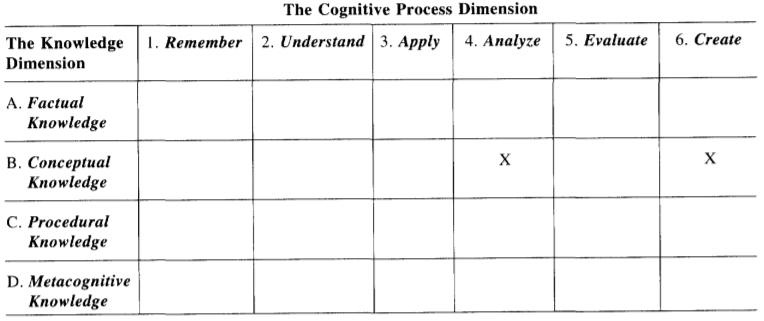
\includegraphics[width=0.9\textwidth]{Figs/blooms.PNG} 
    \caption{Taxonomy Table (Krathwohl 2002)}
    \label{fig:fig2}
\end{figure*}  

\emph{"Is blooms taxonomy appropriate to computer science ?"}, this question has been discussed \cite{johnson2006bloom} and it has been observed that it can be difficult to decide upon which cognitive level a certain task lies at, as educators with a more intimate level of the course material are likely to associate a different level with a task than an educator who does not. This has been discussed further by (Thompson et al. 2008)\cite{thompson2008bloom} who addressed this issue and noted that there hadn't been an agreed upon interpretation of blooms taxonomy for computer science so attempted to do so for a programming module, it was concluded that once staff involved in the teaching of the course an agreement could be made on which cognitive levels tasks belonged to which suggested that the revised blooms taxonomy could be effectively used in the programming domain with regards to exam questioning. Trying to cover all the cognitive levels in an examination however could end up making the exam longer than needed so it has been advised \cite{scott2003bloom} to combine multiple cognitive levels in one question to solve this problem. 

Niekerk and Solms discuss applying blooms taxonomy to information security education and how it can improve security educational programs. They raise potential issues such as that a program that has not been tailored to the specific needs of an individual, or the needs of a specific target audience will be ineffective. They also give an example of how to apply blooms to information security saying that teaching a student what a password is would lie on the \emph{remember} and \emph{understand} level of blooms taxonomy, however, the necessary information to understand  why their own password is needed in order to safeguard might be as high as the \emph{evaluate} level of the taxonomy \cite{van2009using}. An example of blooms taxonomy applied to information security is shown (see Figure \ref{fig:fig3}).  

\begin{figure*}[h]
    \centering
    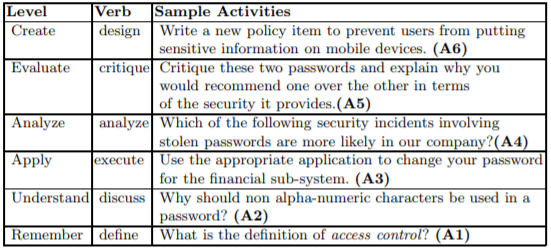
\includegraphics[width=0.9\textwidth]{Figs/blooms2.PNG} 
    \caption{Blooms applied to information security (Niekerk and Solms 2009)}
    \label{fig:fig3}
\end{figure*} 

Buchanan et al. have done research into blending bloom's taxonomy and serious game design suggesting that there may be a way to connect game interaction and the learning objective levels of blooms taxonomy concluding serious games are a good medium for this as they allow novice learner to focus on the general concepts and skills of the subject matter, and not become distracted by a tools interface \cite{buchanan2011blending2}. 
\subsubsection{Psychomotor} 
While the cognitive domain relates to strategic business intelligence, prudence and applying the psychomotor domain relates to complex overt response, Modus (way in which anything is done) and guided response, essentially cognitive is thinking and psychomotor is doing \cite{schutte2016development}. Psychomotor is relating movement or muscular activity associated with mental processes, Psych meaning mind and Motor referring to the motorneuronal system in the brain and spinal cord \cite{tan2007psychomotor}. 
 
Psychomotor skills and computer games have been widely researched over the last 20-30 years for example in teaching psychomotor skills in the medical industry using virtual reality \cite{westwood1998validation} \cite{gallagher2001objective} \cite{gallagher2002virtual} \cite{grantcharov2004randomized} \cite{lehmann2005prospective}. These computer simulation games have been found to improve psychomotor skills \cite{mitchell2004use}. It has been suggested that psycomotor speed can lead to a fast and accurate performance in cyber operations \cite{campbell2015identifying}, psychomotor skills and gaming have been linked with one study suggesting that its likely that frequent and repetitive game playing can improve psychomotor abilities \cite{kennedy2011video}.



\subsection{CTF platforms}
As previously discussed Capture the flag competitions are becoming more and more popular. They consist of a set of challenges each from a different area of cyber security, some of the areas covered include: 
\begin{itemize}
  \item Cryptography
  \item Exploits 
  \item Forensics 
  \item Networking 
  \item Reversing 
  \item Stenography  
  \item Web
\end{itemize}
Cyber security skills will have to be used in different challenge scenarios to find the flag, which will usually be text that can be submitted to a scoring server\cite{burket2015automatic}. Typically these platforms will also have features such as a hint system where a user can get help if they are stuck on a challenge and a scoreboard where users can see who is performing best in the competition.   

\subsubsection{Existing CTF platforms}  
A variety of platforms have been developed to host CTF tournaments, each have their own advantages and are useful for different situations.  
\textbf{CTFd} 
The CTFd framework focuses on ease of use and customisability.  Written predominantly in python. It handles Static and regex-based flags. Users can access hints if they are stuck on challenge. File uploads to the server on Amazon S3. Includes features such as Dynamic scoring, Score graphs, team management and hiding. CTFd also allows users to customise everything using plug in and theme interface \cite{ctfd}.   

When running a CTF using this platform the admin can observe the performance of the participants easily using a statistics page, which tracks things such as the ratio of correct submissions to wrong submissions. The admin can also check the teams, scoreboard and customise the configuration. This flexibility of content creation is CTFd's strength and makes it ideal for changing for intended purposes such as training \cite{noor2018usability}. The user interface for ctfd is relatively simple (see Figure \ref{fig:fig4}).

%% Where is the reference for this
\begin{figure*}[h]
    \centering
    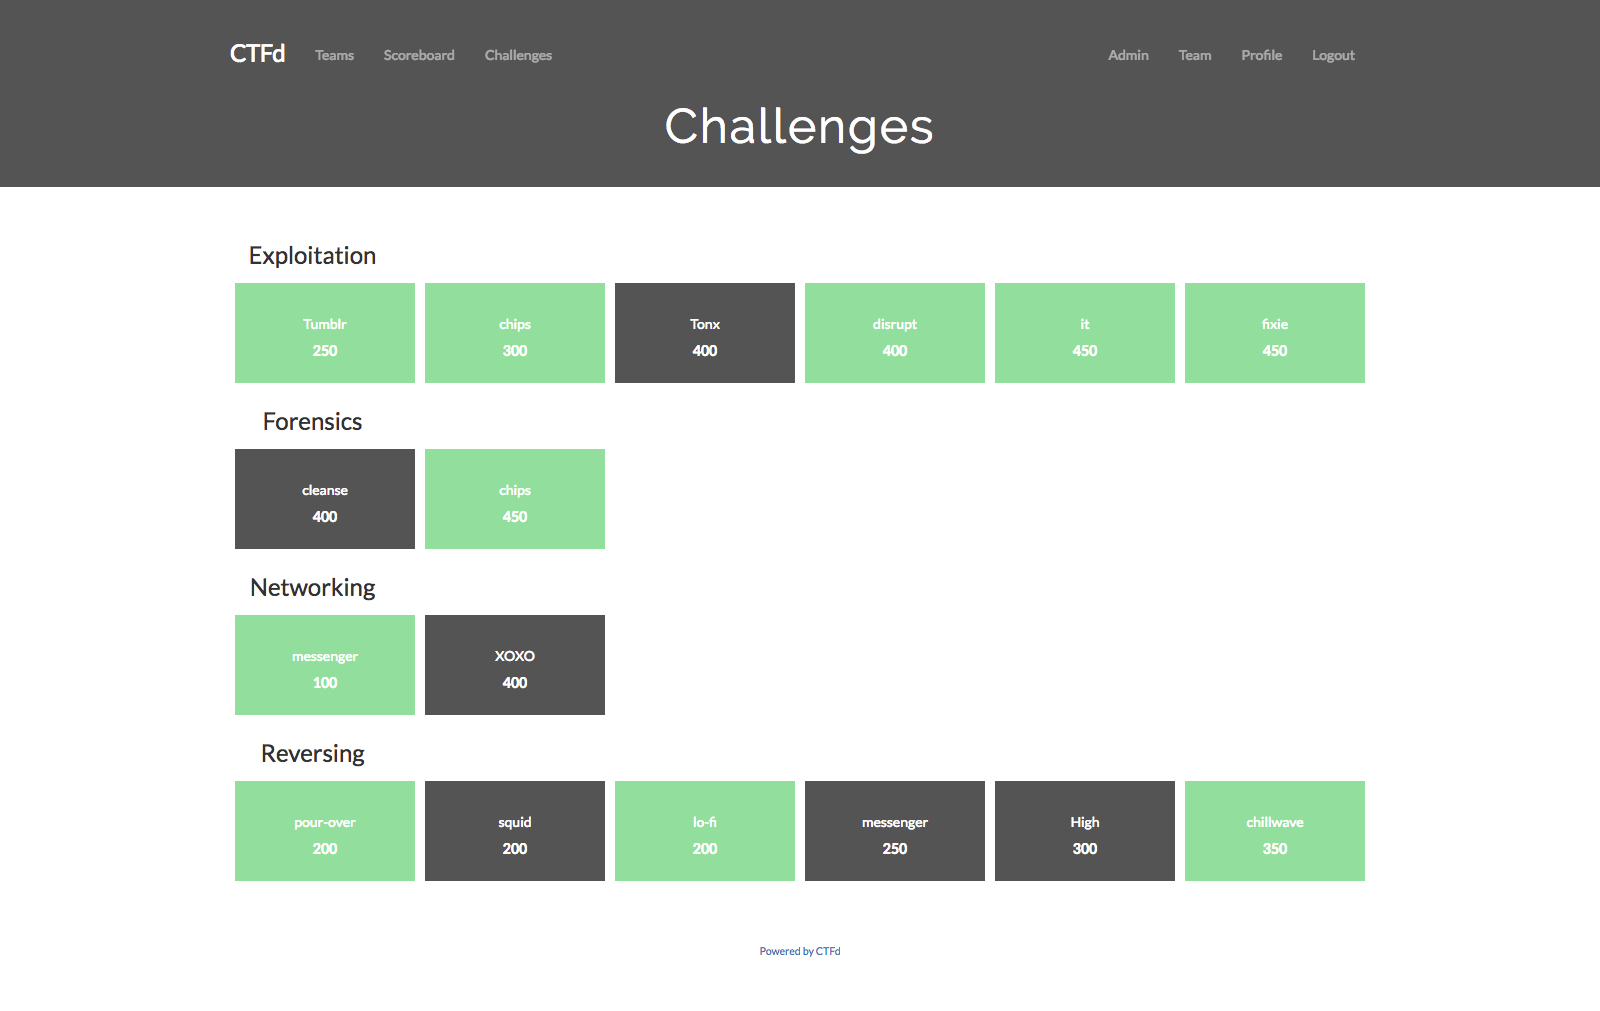
\includegraphics[width=0.6\textwidth]{Figs/ctfd.png} 
    \caption{CTFd User Interface}
    \label{fig:fig4}
\end{figure*} 

As mentioned the CTFd framework is highly customisable allowing the core code to be altered for specific purposes as plug ins, some that have already been developed include: different question formats such as multiple questions, different scoreboard formats and ctf event countdown timers \cite{ctfdplugin}. After downloading the platform you can set up a CTF event, logging in to an admin account on the CTF allows you to easily create your own challenge, setting the category of the challenge the type of flag (e.g static or regex) and what the flag is. The customisation allows the creation of new routes, modifying existing routes, Add tables to the database, registering asset types and challenge type creation \cite{ctfdplugin2}.     


\textbf{Facebook CTF} 
Used for hosting jeopardy and \emph{king of the hill} style CTF competitions. Written in Hack. Can be two players up to several hundred. It has a fancy AI showing a world map, each of the challenges appear in different countries and users will beat the challenges to claim that country. Can be installed in either development mode or production mode. Capturing the countries give you points, you accumulate points which can be compared against other teams/players using a dynamic leader board (see Figure \ref{fig:fig5}) \cite{fbctf}.  

\begin{figure*}[h]
    \centering
    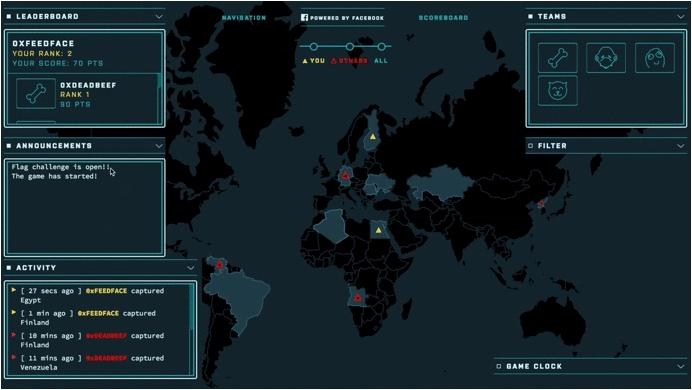
\includegraphics[width=0.6\textwidth]{Figs/fbctf.jpg} 
    \caption{Facebook CTF visualization}
    \label{fig:fig5}
\end{figure*}   

Facebook does not emphasize on customizing the platform as much as ctfd. The platform allows the adding of challenges as an admin by giving a title, question, answer, points, hint, hint penalty and what country on the map the challenge will be placed on but not as much is given with the install to actually change the platform for personal use. Also accessible as an admin is the ability is configuration, controls, announcement and team management where teams can be monitored and given admin privileges. The platform does allow for new pages to be inserted by editing the IndexController file that is included with the initial install. 

\textbf{Mellivora} 

CTF engine written in PHP. Includes features such as arbitrary categories and challenges, scoreboard with optional multiple team types, challenge hints, team progress page, local or amazon s3 challenge file upload and user/email/IP search\cite{mellivora}.  

\textbf{Other CTF platforms and technologies}  
With CTF's gaining in popularity there has been an abundance of applications developed to aid CTF competitions. These range from scoring servers such as Hack the Arch \cite{HackTheArch} which has an optimal dynamic hint system included or Security Scenario Generator (SecGen)\cite{SecGen} which creates vulnerable virtual machines so students can learn security penetration testing techniques, it has been successfully used to enhance security education by providing these randomized targets for lab exercises, large team project security audits and for genrating CTF competition VMs \cite{schreuders2017security}. There are also some "always online ctf's" like Hack the Box \cite{HackTheBox}, ctfs.me \cite{ctfs} and Hone your ninja skills \cite{Ninja} all of which offer challenges similar to ones in CTF competitions available all the time on websites. 


\subsubsection{CTFs in the classroom}
CTFs (class capture the flags) have been researched \cite{mirkovic2014class}, small scoped competitions engaging students in attack and defence scenarios as teams reporting back that this spiked students interest in learning and allowed them to master skills discussed in lectures and introduced in practicals (for suggested differences between a competition CTF and a class CTF (see Figure \ref{fig:fig6})   

\begin{figure*}[h]
    \centering
    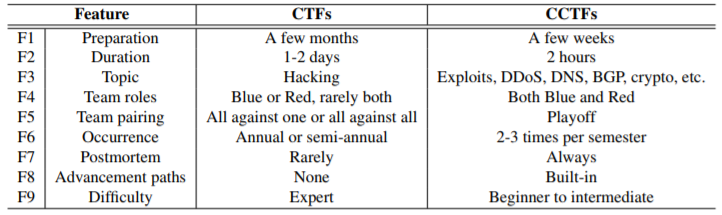
\includegraphics[width=0.9\textwidth]{Figs/cctfs.PNG} 
    \caption{Comparison of CTFs and CCTFs (Mirkovic, Peterson 2014)}
    \label{fig:fig6}
\end{figure*}    

Capture the flag platforms are being used in the classroom for networking \cite{prabawa2017using}, presenting labs in a CTF game with the materials being transferred into challenges, reporting back an increase in the students comprehension skills as well as being eager and motivated to learn. CTFs have even been used by the united states air force academy for teaching cyber security \cite{carlisle2015using} citing students pushing their own boundary for knowledge as an advantage and state they are looking how to further incorporate CTF into their curriculum. CTFs are a thorough security exercise that integrates well with cyber security educational targets and so can be used effectively to train cyber security professionals \cite{eagle2004capture1} as well as an attractive and effective way to raise awareness and interest in security while simultaneously educating for prevention and addressing the private and government sector needs \cite{albert2010high3}. The competitive element of these events drives and compels all participants to more enthusiastically commit and engage in active experimentation and learning \cite{albert2010high5}, this freedom is a key part which motivates students to experiment and forces those students to hone skills that are not normally covered in a standard information security curriculum \cite{eagle2004capture2}. Albert et al performed a study and gathered results by doing a survey, the majority of comments indicated that the students enjoyed themselves and learned more about a field they were interested in and was successful in educating high school students about higher education opportunities \cite{albert2010high6}. 

\subsection{Gamification}
Gamification is the design approach of utilising gameful design in various contexts for inducing experiences familiar from games to support different activities and behaviours and has continued to be a popular topic in both industry and academia since it became popular in the early 2010s \cite{majuri2018gamification}. Gamification has been shown across multiple levels of academic instruction to have a positive impact on task completion by augmenting the experiential elements encountered by students who are engaging in the learning process \cite{kaufmann2018reflection}.



\subsubsection{Gamified elements vs. Gamified experience}
Gamification has been defined as "the use of game design elements in non-game contexts" \cite{deterding2011gamification}. It is important to know when considering the gamification of learning there is a difference between gamifying a whole experience and adding gamified elements. Gamifying an experience involves an actual game, there is a start state, gameplay and an end state. Users can tell they have reached the end when there is a "win state", a long the way the game will have taught some knowledge and skills to the user. Gamifying elements, however, only uses elements of a game. Users will not play through a game start to finish, rather, participate in game elements such as completing challenges or earning points or badges for completing those tasks \cite{kapp2012}.  


The term serious game is given when a complete game is used for a non-entertainment purpose, whereas gamified applications use elements of games that do not give rise to entire games \cite{deterding2011gamification}. Further distinctions between the two have been made, Serious games are usually made to fulfill the role of the tutor providing the instructional content to the learners, gamifying elements on the other hand is designed to augment or support pre-existing instructional content. Furthermore serious games serious games use all game elements just to varying degrees, whereas gamifying elements
involves the extraction and application of particular elements from games for a considered use on a non-game process\cite{landers2014developing}.  

\subsubsection{Game Design} 
Looking more into developing a game for educational purposes, game design needs to be extensively looked at. Games have the ability to provide a media for delivering training in an engaging format at levels appropriate for the individual user \cite{nagarajan2012exploring1}, the idea is also not a new one, games have been used to support health, education, management and other sectors have yielded positive results \cite{prensky2003digital}. When designed well, video games can enthrall players. drawing them into a virtual world, motivating them and challenging them \cite{nagarajan2012exploring2}, with research also indicating that games can support and enhance learning and training \cite{cone2007video}. Game mechanics should be considered when designing a game, these are essentially the rules of the game and fall into classes such as \emph{Setup, Victory Conditions} (how the game is won) \emph{Progression of play, player actions} and  \emph{game views} \cite{nagarajan2012exploring4}.

Annetta defines 6 principles to follow when designing games for education \cite{annetta2010s1}: Players should have a unique \emph{Identity} in the game world, which in turn allows the user to become more emotionally involved in the game and care about the consequences. This leads to \emph{immersion} which is a heightened sense of presence that means the player being more engaged in the content and motivated to succeed. \emph{Interactivity} involves the player being able to interact with NPCs (non playable characters) , \emph{increased complexity} keeps the player challenged, \emph{Informed teaching} focuses on providing feedback to instructors and the game should be \emph{instructional}. 

Similarly but more specifically, Adams and Makramalla discussed four elements of gamification for cyber security skills training \cite{adams2015cybersecurity1}: \emph{Progress mechanics} related to player motivation through the provision of progress tools such as points, leaderboards and badges, \emph{Player control} (which closely relates to Annetta's Identity principal) the use of a character to engage in the gamified training, \emph{Problem Solving} crucial element in gamification when learning and retaining new information and \emph{Story} (which closely relates to Annetta's Immersion principal) a narrative that is the present to create an attachment or bond between the learner and their avatar, stories also motivate the learner to keep on playing to find out the rest of the story. As well as correlating with Annetta's Immersion principal this element is backed up further by literature, an engaging story line makes the player \emph{want} to play the game \cite{buchanan2011blending1} and can provide a narrative for the game and begin to immerse the players in an alternate world. These games create goals that a player feels motivated to reach \cite{nagarajan2012exploring3} this is beneficial for motivation and the more motivated the student the more likely the educational goals will be achieved \cite{albert2010high1}.   

Also when designing a game for cyber security training it would be advantageous to acknowledge shortcomings of existing cyber security training material such as too many topics being discussed in too little time - users cannot be expected to understand/ retain all of them and a successful cuber security skills training program must be able to do two things: one is get and retain the user's attention for a span of time, and two is to communicate training material to the user effectively in a span of time \cite{nagarajan2012exploring5}. 

\subsubsection{Feedback} 
Hattie and Timperley define feedback as information provided by an agent (e.g teacher) regarding aspects of ones performance or understanding. A teacher or parent can provide corrective information, a peer can provide an alternative strategy etc. Feedback is a consequence of performance \cite{hattie2007power}. Simple feedback helps learners verify the performance expectations, judge their level of understanding and become aware of misconceptions, instructional feedback can also provide clues about the best approaches for correcting mistakes and improving performance. Effective performance provides the learner with verification, a judgement of whether an answer is correct, and elaboration, additional information to help the learner \cite{attali2015effects1}.  

One widely researched area of feedback is multiple choice assessments using immediate feedback. Merrel et al. carried out a study assessing the usefulness of reporting back immediate feedback, allowing for the user to make a second attempt and be rewarded partial credit if answered correctly. The results showed that the average grade went up by nearly 6.57 percent \cite{merrel2015multiple}. Further research has indicates that methods that permit immediate feedback to students during lectures and tests increase more effective long term understanding \cite{roediger2011critical}. Attali performed a study comparing different types of feedback: NF (no feedback), immediate knowledge of correct response (KCR), multiple try feedback with knowledge of the correct response (MTC) and multiple try feedback with hints after an initial incorrect response. The study found that 38 percent of users were able to correct their incorrect answer on the second attempt without a hint but with a hint 52 percent were able to concluding that a hint after an incorrect response was more effective that multiple try without hints and as well as providing an opportunity to understand the initial error, provides more information and a clearer path \cite{attali2015effects2}.      

There are also a multitude of different forms of feedback when it games to games such as losing lives, receiving encouraging messages, or earning rewards (e.g points) \cite{adams2015cybersecurity2}.


\subsubsection{Gamification in Computer Science} 
The features previously discussed, such as a point system and leaderboards, are being implemented in modules of Computer Science as gamification becomes an emerging pedagogical technique. A study was done in 2014 at Alabama A\&M university \cite{fu2016gamification} of students studying Computer Science courses. This study reported a match between the score of virtual points and the final grade for the majority of students. The study also states that this result would make it easier to claim that the gamification mechanism drives student motivation to learn.  

More specifically to cyber security, a study was done at a high school camps launched by Purdue University Northwest in the summer of 2016 and 2017\cite{jin2018evaluation}. This study was done by using four cyber security game based learning applications. The results of this study indicated that the camp had not only enhanced the students understanding of cyber security but also increased their motivation to pursue higher education and careers in the field of cyber security. The game based learning applications used in this study may be closer to a serious game than the gamification of learning but perhaps an emphasis on the game elements is what engaged the younger users so much.  

\subsubsection{Negative affects of gamification} 

It is important when looking into developing learning material using gamification to look at the possible negative effects it can have. One paper \cite{toda2017dark} takes a look at multiple studies done on the gamification of learning (the majority of which were in the computing field) and identified four main negative effects that are possible when using gamification: \emph{Loss of performance} where gamification harms or hinders the students learning process by demotivating them. \emph{Undesired Behaviour} where the gamification caused a different effect on the learning context in which it was applied, as a result of poor planning. \emph{Indifference} where gamification simply did have any impact on the students.\emph{Declining effects} occurring less that the previously discussed effects, this effect is the reported loss of motivation and engagement over time when using the gamified application. The paper concludes that these negative effects are likely due to lack of proper methods/frameworks for planning and deploying gamification in a learning environment. It has also been stated that gamified elements of a course lack alignment to curricular outcomes\cite{gonzalez2017cybersecurity}. Another study, looking more specifically at gamified CTF environment identifies \emph{They aren't calibrated to participants needs, partial credit is typically not supported and the need for expert support personnel} as potential issues \cite{katsantonis2017conceptual2}. 

\subsubsection{User Interface} 
HCI (Human Computer Interaction) focuses on how best to design interactive systems so that they are both productive and as pleasurable to use by the intended user as possible \cite{smith2006human}, getting the user interface right can make a fundamental difference \cite{ritter2014foundations1}. Traditional user interfaces deliver information with a minimum of subtlety and, due to users limited attention capacity, must keep throughput low \cite{bulling2016pervasive}.  One important aspect that should be considered when designing a user interface is consistency, for example can all the pop down menus be easily identified by a shared marker such as a downwards arrow. A menu without such notification would be an inconstancy and could initially confuse the user \cite{nielsen2014coordinating}. A dangerous assumption that is made when designing user interfaces is that 'Everyone is like me', this should be avoided and it should be taken into consideration the gap in understanding between the designer and the targeted user \cite{ritter2014foundations2}. However when designing a user interface with novice users in mind a balance needs to be struck as to support expert users who are often trapped in "beginner mode" \cite{cockburn2015supporting}. Many in the computer field cite different ways to design better user interfaces such as "Know the user", "designers are users too, just give them the space and time to design it" and "make the components good enough and the system will take care of itself" \cite{card2017psychology}.

\subsection{Conclusions}
To conclude, the Cyber Security industry is crying out for professionals who are skilled and experts in their field. Deploying CTF styled learning in a gamified fashion in the classroom could help combat this shortage, with an almost unanimous agreement across many research papers that  the CTF style of learning helps users get to grips with cyber security skills and potentially spark an interest in cyber security. By combining the the two it is possible to take advantage of the benefits of both CTF learning and the discussed benefits of a gamified experience. While the impact of this style of learning should not be underestimated it should also be taken into account that there are potential drawbacks which should be taken into account during the development of the platform. Similarly caution should be taken when developing the learning material, making sure the appropriate levels of the cognitive domain are covered while keeping the questions at an achievable level. While it may not have been clear in the past how to apply certain taxonomies to computer science or how to efficiently use gamified learning in a classroom environment, their use is becoming more and more common and with the popularisation of CTFs as a teaching tool and the benefits of gamified learning being widely discussed solutions are being discovered so that this method of learning can succeed and benefit the cyber security industry.

\newpage
\section{Design}
\subsection{Introduction}   

This chapter of the dissertation contains the design for an application that will take full advantage of the researched areas maintaining the goal of engaging a younger audience with the possibility of developing an interest in cyber security. This chapter of the dissertation hopes to design this gamified application with elements of a CTF competition used in the design process with blooms taxonomy being considered in the design process also. By doing this elements of serious games which research has shown can engage a younger audience using elements such as story and player control, will be combined with the structure of CTFs which competitive nature compels students and freedom of choice encourages students to experiment and learn various areas. As it is designed to be an educational tool the research done on Blooms taxonomy will be applied ensuring the appropriate domains are covered and that the learning element of the application is done at an engaging level and is not overwhelming or boring. Combining these elements into one cohesive application will emphasise gamification, taking advantage of the many positives that research has shown it can have whilst also taking into account the potential pitfalls that can be involved when using gamification as to avoid them. Ultimately the goal of this chapter is to combine the research done in the previous chapter with knowledge of available alternatives to design the concept for an application which is effective in handling complex subjects in a way that younger students can understand and apply the skills after use an additional effect hopefully being, which the research shows is often the case with CTF style learning, an increase in interest for the subject of cyber security itself. 

The literature has backed up the need for such an application, now how the areas covered can be implemented in the design of the application will be looked into and will go on to discuss how the application will be designed in regard to its structure taking account what has been discovered in the literature. The design of some of the lessons that application could contain will be done before then going into detail about the technical design of the application. This will take into account methods of research and consider what the best approach to take is to meet the aims of the project. 

\subsection{Requirements analysis} 
After doing the appropriate research on the topic, and designing the concept for the application how best to carry out the research to meet my aims and objectives was then considered. Williams defines qualitative research as allowing the user to explore and better understand the phenomenon whereas quantitative research provides and objective measure of reality \cite{williams2007research}. Greenbaum has further discussed these research methods \cite{greenbaum1999moderating} and cited Michiello's table as useful for deciding a primary research method (see Figure \ref{Research}). 

\begin{figure}[!hb]
    \centering
    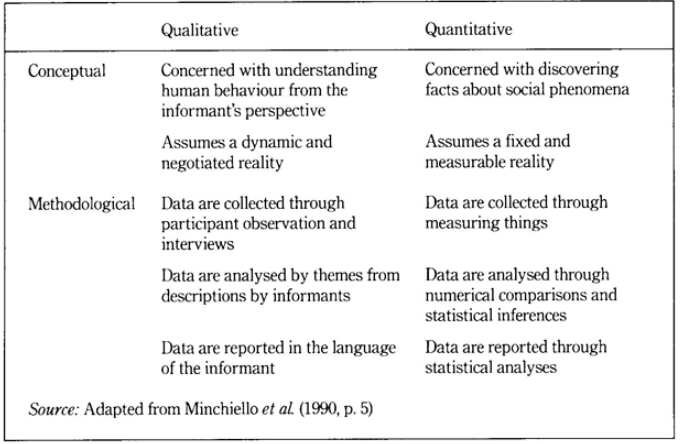
\includegraphics[width=0.75\textwidth]{Figs/research.PNG} 
    \caption{Quantitative vs Qualitative} 
    \label{Research}
\end{figure}  

As the table shows the qualitative method would involve me studying the human interaction side of things, e.g making the application and through the form of questionnaires, getting data on how the application was useful. A quantitative method involves measuring things, numerical comparisons, discovering facts etc This would involve prototyping aspects of the application and measuring their use. Both methods would be valid for meeting the aims and objectives of the project if designed right. However the qualitative method in this case would involve testing the application on the target audience (high school students 
) and would therefore throw ethics into consideration. Another issue with the qualitative method is if this dissertation was planning to do a questionnaire to gather data on the effectiveness of the application, that questionnaire should really have  started to be designed earlier in the project life. The quantitative method however, could be useful in after theoretically designing the app prototyping components of it and gauging how useful it would be in achieving the desired effect by testing and measuring the technical performance of the prototyped components. This would help give insight into the proposed use of the technology and if it should be considered for this use. For this reason it was decided to choose the quantitative method of research and do a technical evaluation on prototyped elements of the proposed application.


\subsection{Application Design}  
To design the structure of the the application, and how the rooms/levels would be spaced out the literature was referred to, to design an application that would effectively teach cyber security skills and knowledge. 

Firstly each “lesson” would be separated into a room in the game. A series of these rooms or “lessons” would make up a floor. These rooms would cover and teach different topics of cyber security. Instead of having floors cover different topics, which is how the application had originally been envisioned, the literature suggests that blooms taxonomy Is an effective teaching model to apply to cyber security education so each floor could represent a different level on the blooms taxonomy (with the exception of the first floor which could combine the first two "remember" and "understand") level of understanding, as the literature suggested there may be a way of blending serious game elements with blooms taxonomy \cite{buchanan2011blending2} this is a proposed way of doing so. So as the user would progress up the floors the questions would get more complex and require deeper thought. For a visual representation of this structure (see Figure \ref{gamearch}).  This would allow the application to impart skills in an organised manor so that the user would get the most out of it and by the end of the application would be at the final level of blooms taxonomy. 

\begin{figure}[h]
    \centering
    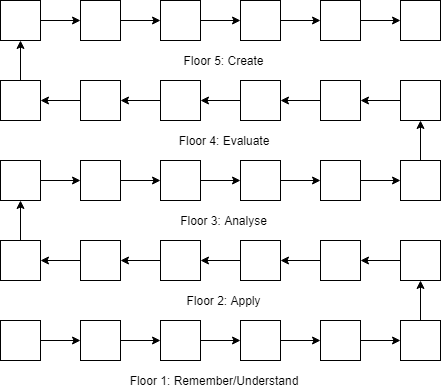
\includegraphics[width=0.75\textwidth]{Figs/gamearch.png} 
    \caption{Proposed Game Architecture} 
    \label{gamearch}
\end{figure}

Another aspect to consider in regards to the structure is that putting “lessons” / rooms back to back requiring the user to complete the lesson in order to progress to the next would be a bad idea. This has been shown to stunt the learning of younger audiences and discourage them from continuing if they can’t get the answer. The literature backed this up implying that freedom of choice is an important factor in gamification and that it encourages the user to explore more and be more engaged with the learning process, with the literature previously discussed saying this freedom motivated students to experiment \cite{eagle2004capture2}. To get around this the application feature something called “reward tokens” which the user would get every time they complete a room/lesson. Say there are 5 rooms on a floor, the user would need to obtain 3 reward tokens to proceed to the next floor. Therefore giving the user the freedom to choose which 3 lessons to complete. The user would also need to be stopped from just all 5 lessons on the first floor then only 1 in the second to progress, a solution to this would be to double the reward tokens the user gets for completing a lesson as the floors ascend and adjust the reward tokens needed to go up a floor according. 



The user would also need to not be discouraged if they for example could only complete two the lessons and is stuck on completing a third on a floor. Having looked over the literature on feedback it suggests that just telling the user that they are wrong isn’t very effective but that giving the user some form of hint is beneficial for the user \cite{attali2015effects2} allowing them to not give up if they don’t know the answer but be pointed in the right direction, with more points being rewarded for an initial correct response and less for a second attempt etc. For this reason a hint system is included in the theoretical design of the application.  If the user unsuccessfully attempts a lesson 3 times then a hint room could unlock. 

The rooms could be designed to incorporate all of these features. In a typical room there would be an opening in every direction. One to the left taking the user to the previous room, one to the right taking the user to the next room, one above which will unlock when the user gets the question right and takes them to the reward room where they can collect the reward tokens and finally one below which would unlock on the third incorrect attempt taking the user to the hint room. For a visual representation of this structure  (see Figure \ref{roomarch}). 

\begin{figure}[h]
    \centering
    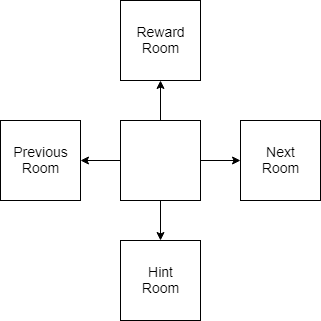
\includegraphics[width=0.75\textwidth]{Figs/roomarch.png} 
    \caption{Proposed Room Architecture} 
    \label{roomarch}
\end{figure}

The user would play as “anonybot” a robot working for moral Corp who when doing his job discovered they were unlawfully harvesting and processing the personal data of customers. When he confronted his superior about it he was locked down on the bottom floor of the headquarters. The user must play as anonybot as he ascends the floors so he can escape the HQ and out the company for what they are doing.

The inclusion of a character, story and an end goal to reach it all factors which have been cited as useful in engaging a younger audience with learning material \cite{adams2015cybersecurity1} (the narrative creating an attachment/bond with the user and avatar), investing them and making them want to reach the end goal by the literature. As this application is aimed at the younger high school audience, with the aim of engaging them in cyber security this is also included in the theoretical design. 

So in summary the application would essentially be a gamified cyber security application, structured similarly to capture the flag (or CTF) events with the freedom of choice operating as the jeopardy style of CTF shown to be effective in engagement, the lessons serving as the challenges and the reward token serving as a flag. The hint system in place is also represented in typical jeopardy style CTFs. The difference is the character and story orientated take and the elevation of floors representing a respective level of Blooms Taxonomy. 
\subsection{Lesson Design}  
As discussed the level design would be rooms bundled into floors, each floor representing a different level of complexity on Blooms Taxonomy. For this design chapter this dissertation will briefly discuss what some of the lessons in the rooms on the first floor would look like, what their content will be, their learning outcomes and then go on to discuss how this dissertation will achieve this. 
\subsubsection{Caesar cipher} 
One of the first things that would be covered in the application is basic encryption types, such as the Caesar cipher.  

\textbf{Learning Outcomes} 
\newline the learning outcomes for this particular lesson would be:  

\begin{itemize}\itemsep0pt
	\item The user would know and understand what a Caesar cipher is 
	\item The user will be able to use an online decoder to get cipher text into plain text
\end{itemize} 

\textbf{Lesson Contents} 
\newline The user would first in a text terminal be told what a Caesar cipher is and would be explained how encryption and decryption work using it. The user would then be given a random Caesar cipher of a famous computer scientist and told to open a online decoder. Using the decoder and referring to the provided steps the user will be able to get the plain text and when entered in the terminal would unlock the door.

\textbf{How this would be done} 
\newline Dynamic challenge generation is an important part of this application and would ensure that the students all have a unique experience meaning users can't copy off of each other's answers and will have a different experience if playing again. This is discussed furthermore later in the design chapter. For this lesson test scenarios would be made using random selection and API requested methods, these will also be discussed further later in the design chapter. 

\textbf{How it would look}  
The caesar cipher lesson has been mocked up (see Figure \ref{caesarmock}).
\begin{figure}[h]
    \centering
    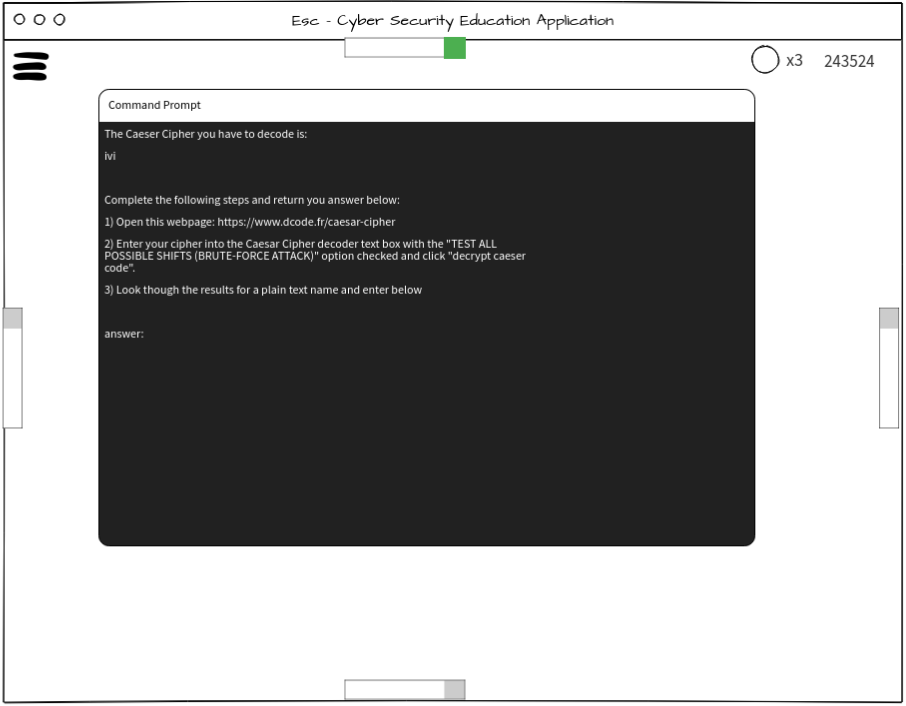
\includegraphics[width=1.0\textwidth]{Figs/caesermock.PNG} 
    \caption{Caesar Lesson Mock up} 
    \label{caesarmock}
\end{figure}   


 


 
\subsubsection{Hash crack}   
Another lesson that would be covered on the first floor of the application is hashing. 

\textbf{Learning Outcomes} 
\newline the learning outcomes for this particular lesson would be:  

\begin{itemize}\itemsep0pt
	\item The user would know and understand what a hash is 
	\item The user will be able to use the command line 
	\item The user will, with instructions, be able to crack a hash using a dictionary and john the ripper. 
\end{itemize} 

\textbf{Lesson Contents} 
\newline The user would first in a text terminal be told what a hash is, about one way encryption and the use of it. Then the user will be taught briefly about the command line, basic commands and about john the ripper. the user will then get given a famous computer scientist hashed and be guided with a set of instructions on how to run the hash against a dictionary of computer scientist to get a match using john the ripper. Once the user find a match they will enter it and the door will unlock.

\textbf{How this would be done} 
\newline For this lesson the test scenarios would be made using the web scraping method, this will also be discussed further later in the design chapter. The lesson would then have a dictionary full of the hash value of different computer scientist provided to the user.  

\textbf{How it would look} 
This lesson would look the same as the caesar lesson, with the lesson being done over the command line.
 

\subsubsection{Who is this ?}
%discuss the learning outcomes e.g teach young audience maybe who some famous computer scientists are and why they are famous. Discuss how i will make it get progressively harder until at the end they win reward token. mock up how will look. Discuss how i will use face api, bing api and webscraping to do this.  

Also a possible lesson on the first floor would be a simple "which one of these images is...." stage, asking the user to identify a computer scientist out of a selection of pictures.  

\textbf{Learning Outcomes} 
\newline the learning outcomes for this particular lesson would be:  

\begin{itemize}\itemsep0pt
	\item The user will be able to recognise famous computer scientists.
\end{itemize} 

\textbf{Lesson Contents} 
\newline The user will be presented with a question "which one of these people is *insert person here*" , four pictures will then be displayed on the screen, one being the right person and one the three others being other computer scientist. When the user gets this right they will proceed to stage 2 and be asked again, this time it will be slightly harder, a less famous computer scientist. Finally if they get that correct they will proceed to the third stage with a lesser known computer scientist. By answering the third question correct the lesson would be complete and the door would unlock. An incorrect answer will result in the user having to go back to the first stage again, this is multiple choice with immediate feedback and has been discussed and backed up by the literature \cite{roediger2011critical}. This technique of try and try again has been shown to be effective for imparting knowledge. 

\textbf{How this would be done}  
\newline For this lesson the test scenarios would be made using the web scraping method with the use of two API's, which this dissertation will go into more detail about later in this chapter.  

\textbf{How it would look}  
The "who is this" lesson would show four images on the screen and ask "which one of these picture is Alan Turing" for example the user would select one of the four pictures and depending on whether they were correct or not the stage counter would change (see Figure \ref{facemock}).
\begin{figure}[h]
    \centering
    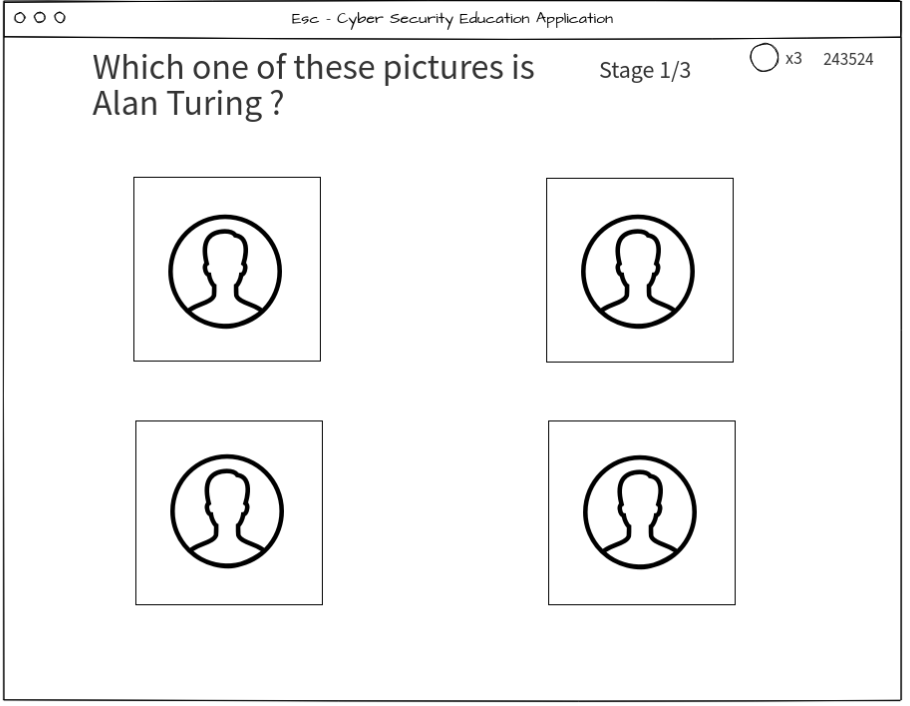
\includegraphics[width=1.0\textwidth]{Figs/facemock.PNG} 
    \caption{Face match Lesson Mock up} 
    \label{facemock}
\end{figure}  


\subsection{Technical Design}  
This section of the dissertation covers the design of the technical elements of the project, starting with mocking up the user interface, then designing the methods of dynamic challenge generation and finally a discussion on the back end of the proposed application designing databases. 

\subsubsection{Front end: User Interface}  
The user interface will take into account the literature and represent the application in the most effective way possible. The main screen would be relatively simple (see Figure \ref{Mainscreen}).

\begin{figure}[h]
    \centering
    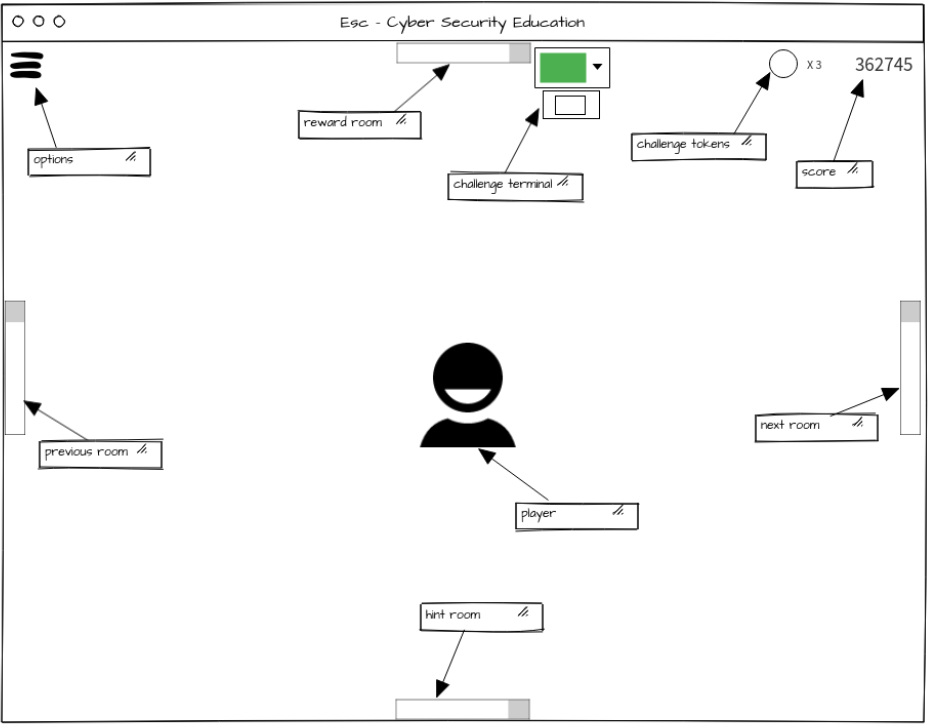
\includegraphics[width=1.0\textwidth]{Figs/Ui_main_screen.PNG} 
    \caption{Main Screen UI mock up} 
    \label{Mainscreen}
\end{figure}   

The main screen has quite a lot going on. In a typical room, the player will have a choice to navigate both to the next room and the previous room to their left and right. If they go up they will reach the challenge terminal which when interacted with brings up the challenge. If they enter the correct answer the reward room will open up and they can collect their challenge token. If they get it incorrect the hint room below opens up. How many Challenge tokens they have is displayed and also the score they have accumulated so far. The user can quit or alter their settings with the drop down menu in the top left hand corner of the screen (see Figure \ref{Mainmenu}). The idea of the design was to try and cover all the necessary elements of the application but keep everything consistent and keeping the delivery of information clear and apparent as per the literature's suggestion \cite{bulling2016pervasive} \cite{nielsen2014coordinating}. 

\begin{figure}[h]
    \centering
    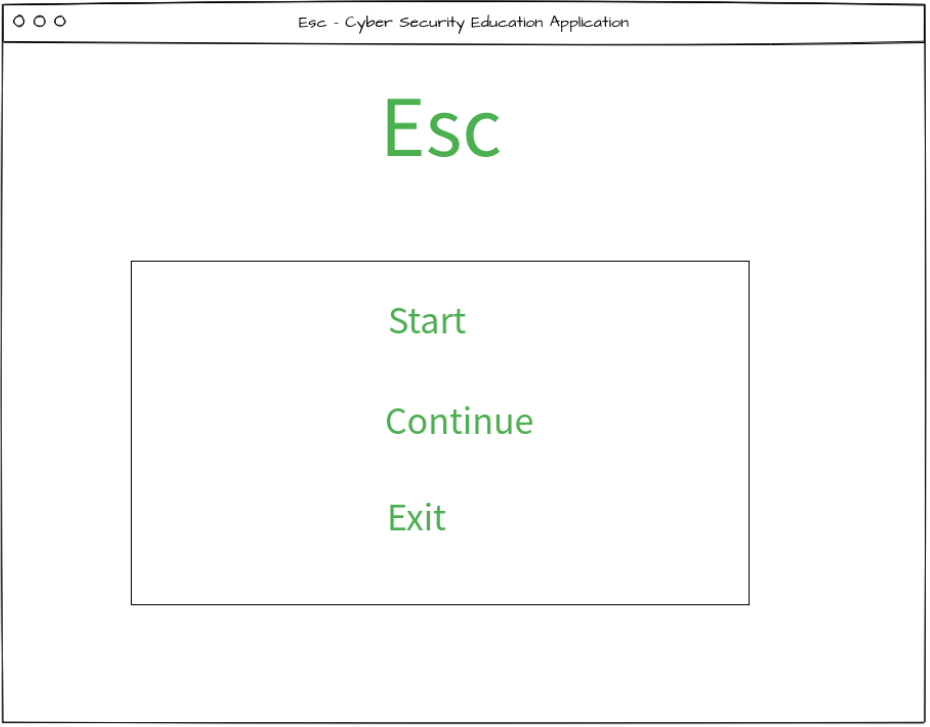
\includegraphics[width=1.0\textwidth]{Figs/Ui_main_menu.PNG} 
    \caption{Main Menu UI mock up} 
    \label{Mainmenu}
\end{figure}   

\begin{figure}
\centering
\begin{minipage}{.5\textwidth}
  \centering
  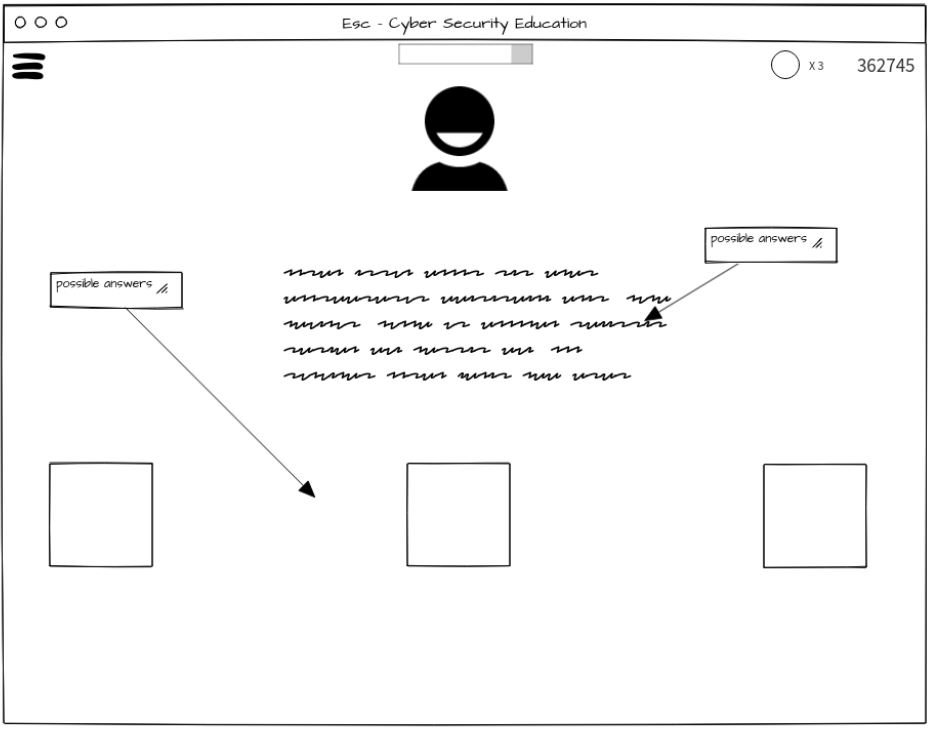
\includegraphics[width=1\linewidth]{Figs/Ui_hint_room.PNG}
  \captionof{figure}{Hint room}
  \label{fig:test1}
\end{minipage}%
\begin{minipage}{.5\textwidth}
  \centering
  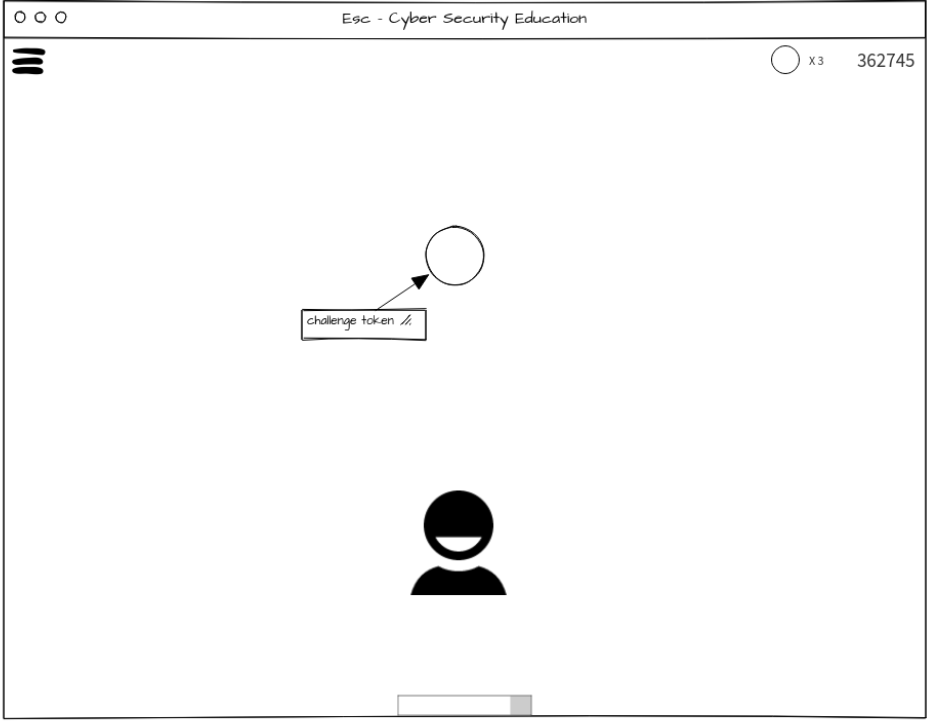
\includegraphics[width=1\linewidth]{Figs/Ui_reward_room.PNG}
  \captionof{figure}{Reward room}
  \label{fig:test2}
\end{minipage}
\end{figure}   

When the user enters the hint room they are presented with a question and a choice of three answers (see Figure \ref{fig:test1}). They will get the hint regardless but is meant to build their knowledge and whats been covered. The reward room is simple and just contains the challenge token (see Figure \ref{fig:test2}). 

\begin{figure}
\centering
\begin{minipage}{.5\textwidth}
  \centering
  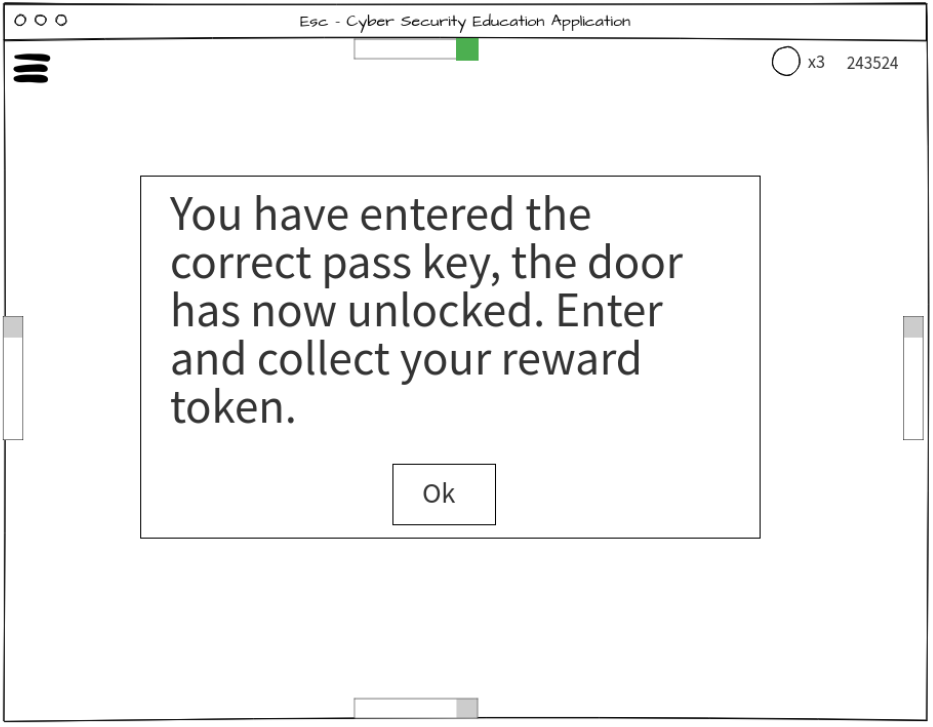
\includegraphics[width=1\linewidth]{Figs/Ui_correct_response.PNG}
  \captionof{figure}{correct response screen}
  \label{fig:test3}
\end{minipage}%
\begin{minipage}{.5\textwidth}
  \centering
  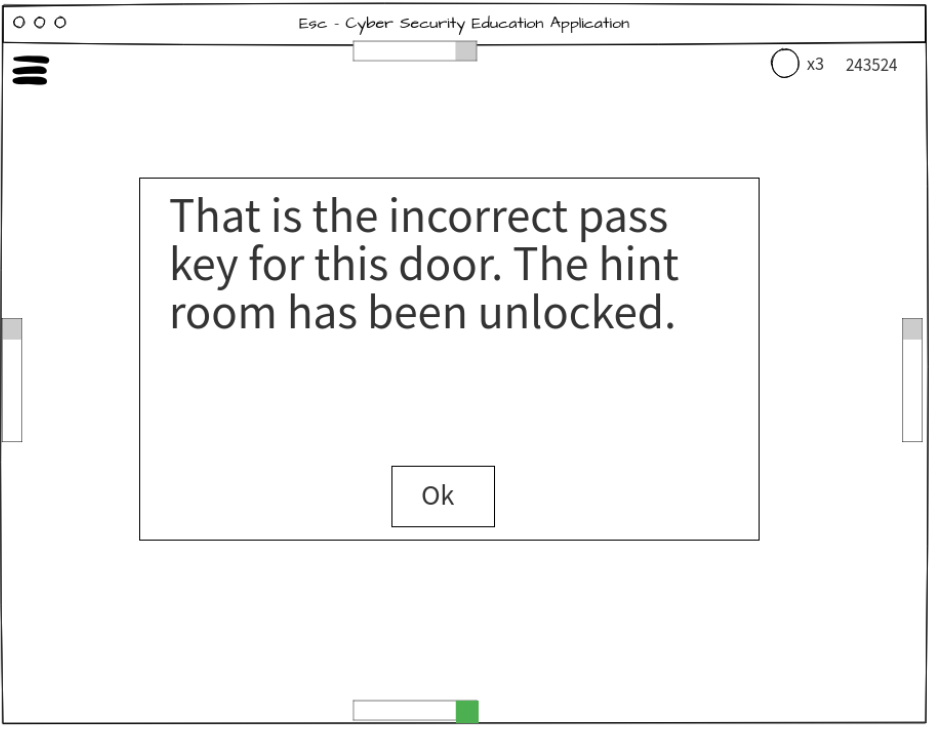
\includegraphics[width=1\linewidth]{Figs/Ui_incorrect_response.PNG}
  \captionof{figure}{incorrect response screen}
  \label{fig:test4}
\end{minipage}
\end{figure}  

The feedback received at this level is basic, keeping throughput to a minimum was encouraged and backed up by the literature \cite{bulling2016pervasive}, dependent on what the answer is different doors unlock (see Figures \ref{fig:test3} \ref{fig:test4}).



\subsubsection{Middle end: Dynamic Challenge generator}  
One fundamental part of this application will be the challenge generator. Dynamic challenge generation is an important element of this application, it will ensure that if the user comes back and does it again they will have a different experience and also that users will be having a different experience than the users around them. This dissertation will look at three possible methods of dynamic challenge generation. \emph{Random challenge selection, API request} and \emph{Web scraping}.  

\emph{Random Challenge selection} 

This will involve setting up a list of possible questions with corresponding answers, then selecting one of those questions at random. A multiple choice question would be asked populated with the correct answer and the answers to the other questions. The script would them check for the user input and check if the answer matches the correct answer giving simple feedback accordingly. This will be the simplest method and the easiest to implement (see Figure \ref{RandomSelection}).  

\begin{figure}[h]
    \centering
    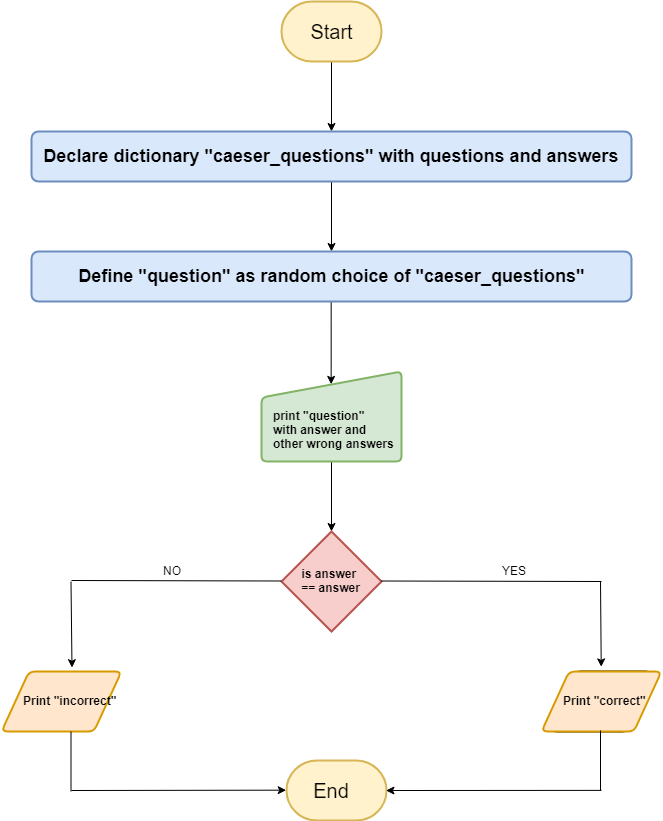
\includegraphics[width=0.5\textwidth]{Figs/random_selection (1).png}
    \caption{random selection flow chart} 
    \label{RandomSelection}
\end{figure}   


\emph{API request} 
An API will be set up using a python script so a request can be made to it with another script. The script will select a random word from a list, the world will correspond with a question that the API will send back when it receives this word. The user will then send back the answer which will be sent to the API and checked (see Figure \ref{APIRequest}).   

\begin{figure}[h]
    \centering
    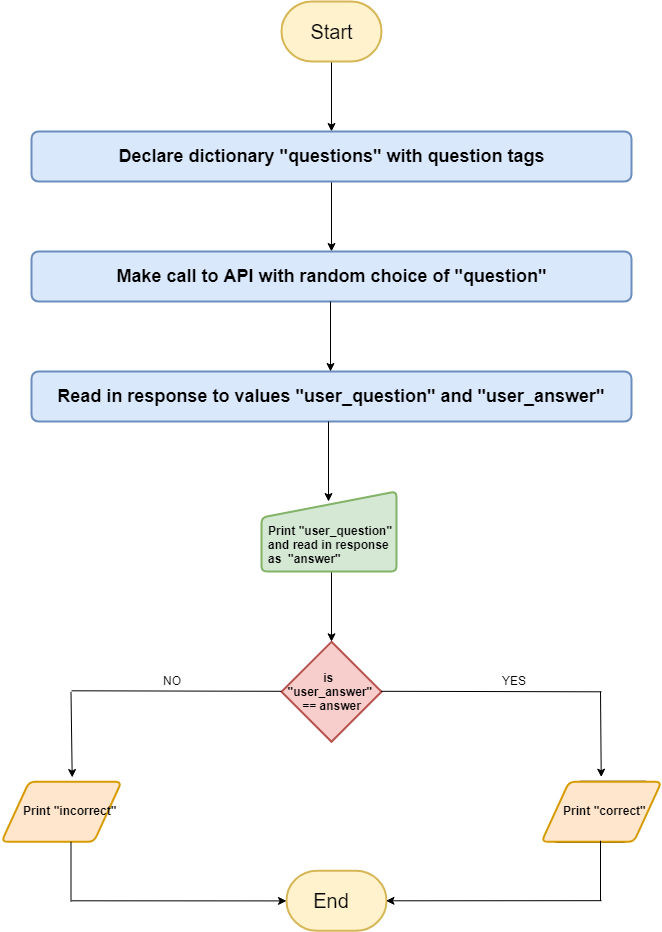
\includegraphics[width=0.5\textwidth]{Figs/API_request.png} 
    \caption{API request flow chart} 
    \label{APIRequest}
\end{figure}   


\emph{Web Scraping} 
Two web scraping applications will be developed to test the effectiveness of it as a method of dynamic challenge generation, one simpler one and one more complex. For the more simple one the names of influential computer scientists will be scraped from sites like either 'https://www.computerscie
ncedegreehub.com/30-most-influential-computer-scientists-alive-today/' this or a Wikipedia entry on something similar. Then will read those names into a list. The challenge would be generated by grabbing a random name from that list and running it through an online hash generator, providing all the information you need for the challenge (see Figure \ref{WebScraper}).   

\begin{figure}[h]
    \centering
    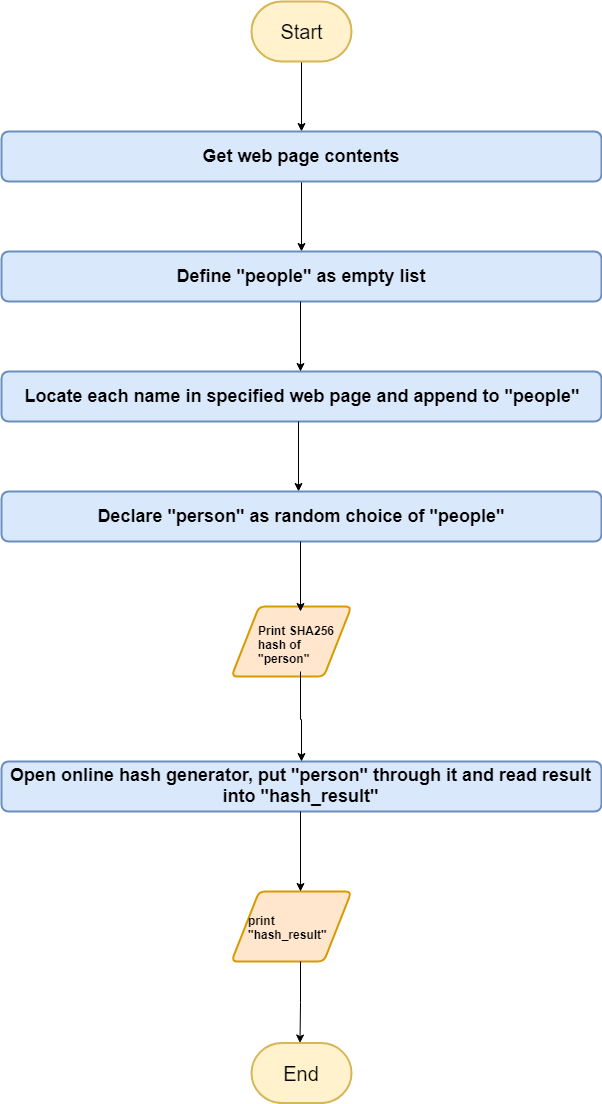
\includegraphics[width=0.5\textwidth]{Figs/Web_scraper.png} 
    \caption{Web scraper flow chart} 
    \label{WebScraper}
\end{figure}   


The more complex use of web scraping would involve using the Bing API and the Microsoft cognitive engine. The script would ask the Bing API for 100 cryptographers, it would then store images of them in a list, returns one at random and sends it to the Microsoft cognitive engine to see if it recognised it. This script would be used to ask the users if they recognise the famous cryptographers and check their answer against the answer returned from the Microsoft cognitive engine (see Figure \ref{FaceQuiz}).   

%talk more about how it would work and then make diagram showing how it works%
\clearpage{}

\begin{figure}[!ht]
    \centering
    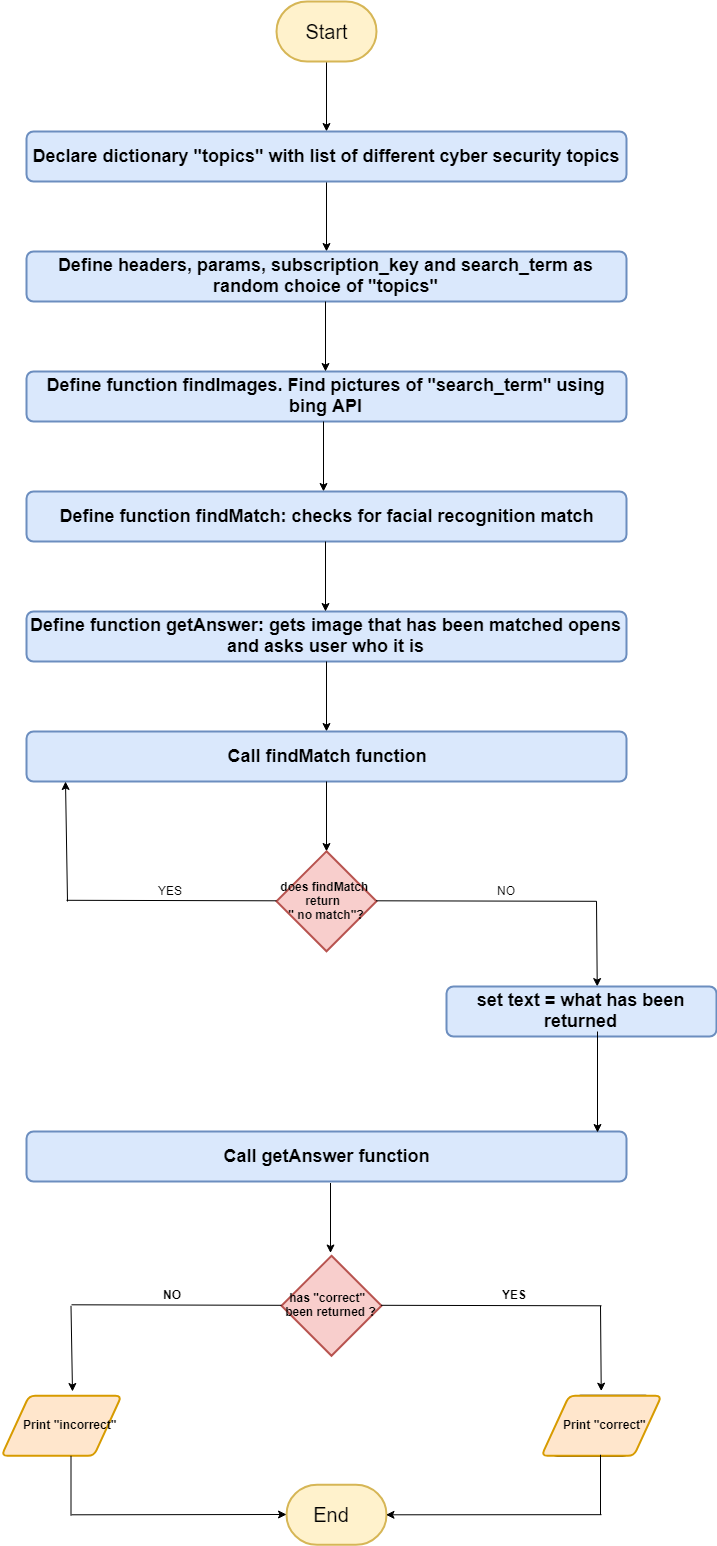
\includegraphics[width=0.50\textwidth]{Figs/Face_Quiz (1).png}
    \caption{Face Quiz flow chart} 
    \label{FaceQuiz}
\end{figure}     

So the script would select a random search term from a list of possible topics. It would then make a call to the Bing API which will return 100 images of the search term. One of these images will be selected at random and be sent to the Face API, the Face API sends the response back in a JSON format. This will loop until a match is found and the Face API matches a name to the face, when a match has been found the image is displayed and the user will be asked who it is (see Figure \ref{APIstructure}).  

\begin{figure}[!ht]
    \centering
    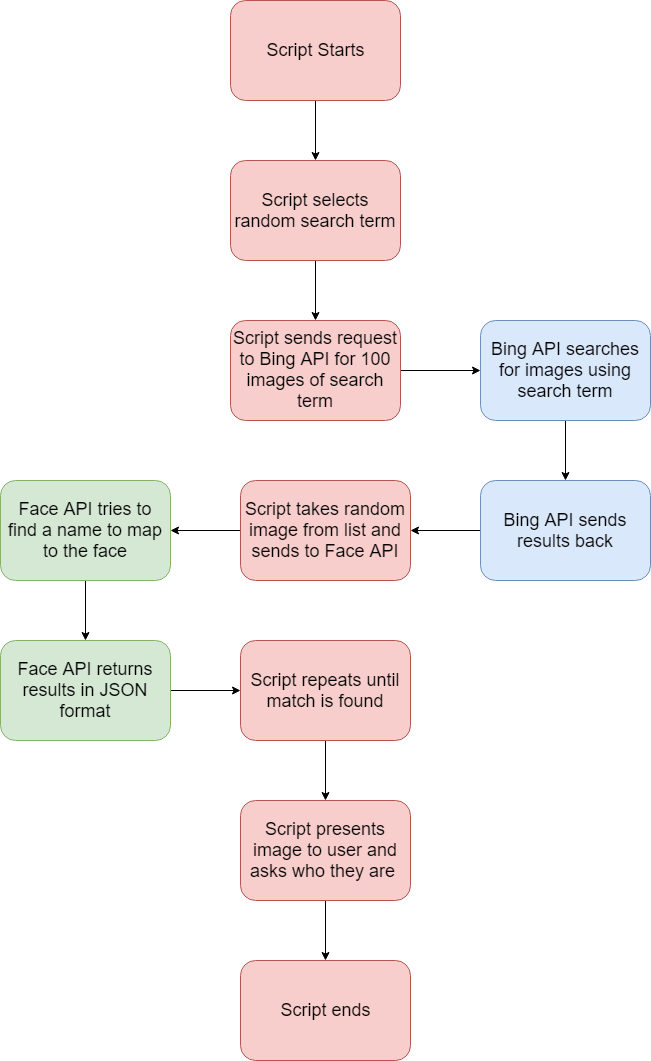
\includegraphics[width=0.50\textwidth]{Figs/API_structure.png} 
    \caption{API structure} 
    \label{APIstructure}
\end{figure}   

\emph{Docker} 
%talk about use of docker and include figure showing how the api is going to be used to send data to database  
 
Docker is a way of systematically automate the faster deployment of applications using portable containers. Docker containers are created using base images, images are created manually are with Dockerfiles. Dockerfiles contain instructions to be automatically performed. They are used to organise deployment artefacts and simply the deployment process \cite{bernstein2014containers}. This service will be used to populate the challenge database. This will be done by making a script (similar to the Face Quiz script) that instead of opening an image and asking the user who it is being displayed, when a match is found inserts into the challenge database the "question" ("who is this ?"), the image url and the answer (the name of the person) (see Figure \ref{DockerFace}) This would be all that is needed to populate the challenge database ( see Figure \ref{Dockerstructure}). A Dockerfile was set up to run this script and insert data into the database. Then using docker X amount of containers could be spun up and the database would be populated with X entries (see Figure \ref{Dockerexample}). By designing it in this manor the database of challenges could be populated in a fast and efficient manor, which would also save processing time when retrieving challenges instead of having to perform the facial matches and image searches at the time of running the script the script could then just retrieve a set of images from the challenge db.
 


\begin{figure}[!ht]
    \centering
    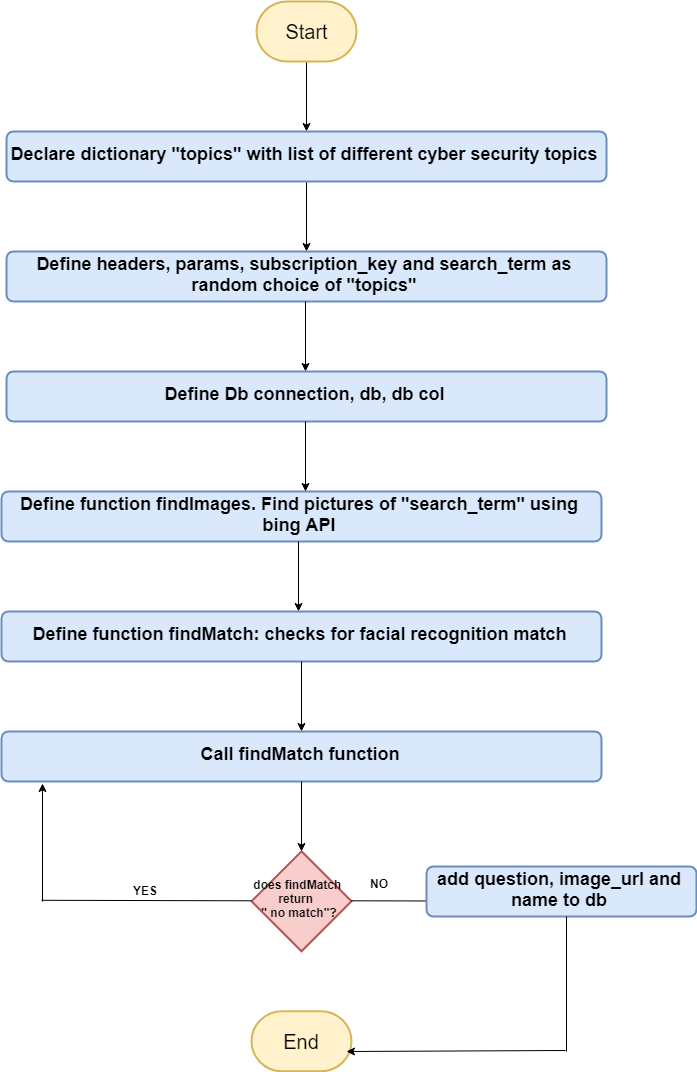
\includegraphics[width=0.5\textwidth]{Figs/Docker_face_pop.png} 
    \caption{Docker face pop flow chart} 
    \label{DockerFace}
\end{figure}     

\begin{figure}[!ht]
    \centering
    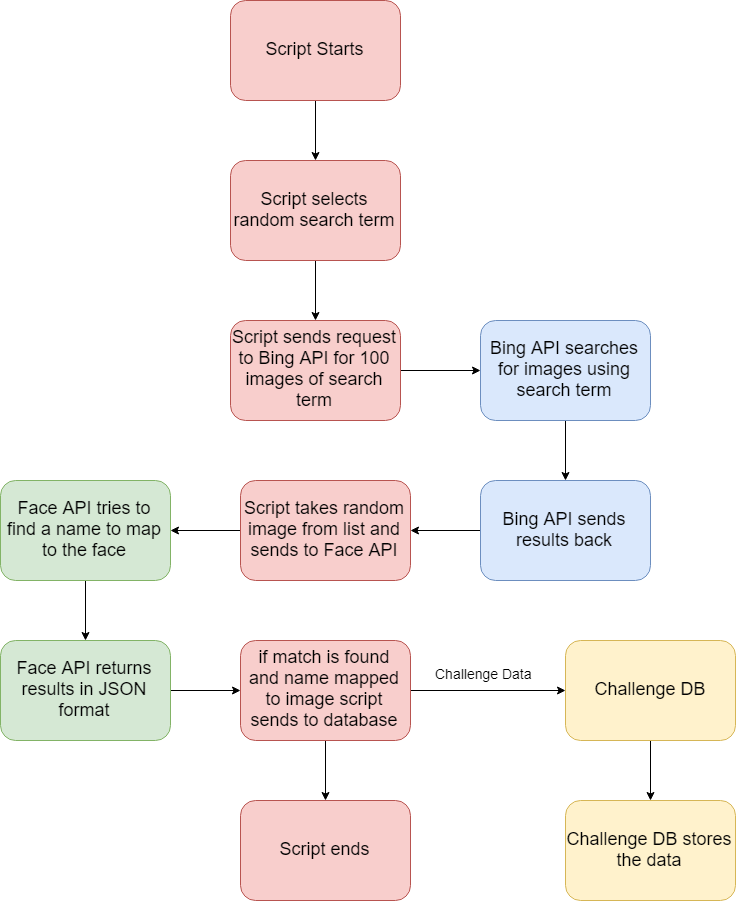
\includegraphics[width=0.50\textwidth]{Figs/Dbinsert_structure.png} 
    \caption{Database population structure} 
    \label{Dockerstructure}
\end{figure} 

\begin{figure}[!ht]
    \centering
    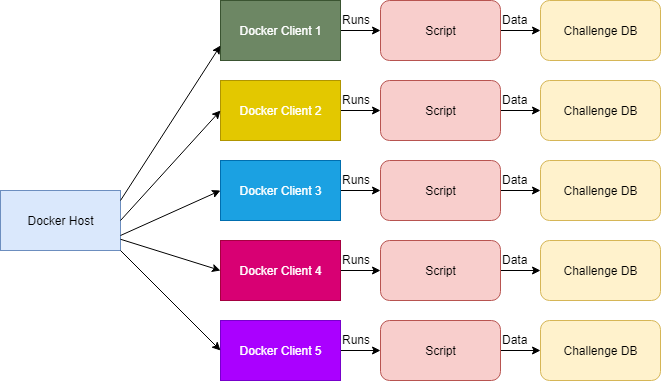
\includegraphics[width=0.50\textwidth]{Figs/Docker.png} 
    \caption{Docker Container example} 
    \label{Dockerexample}
\end{figure}

\subsubsection{Back end: Databases} 
\textbf{SQL vs NoSQL}   
First off when designing the back end of an application what Database would be most efficient to use for the applications specific needs and potential uses. As this application would ideally be scalable and have data being inserted and taken out at high speeds if it was scaled, it made sense to design choose to use NOSQL over SQL with NOSQL growing in popularity because of its ease of access, speed and scalability \cite{li2013performance}. Database management is very important when considering scaling because a lot of the load comes from complex queries making results take longer, so techniques such as caching complex query results and effective organising of db tables with keys and index can be effective in reducing load.
 

\textbf{User Database}   
The user Database would be built to service pupils to make an account. So they can register at the beginning and have a score associated with it. Each user would have a username which would be stored in plain text and a password that would be stored as a hash, then a salt that would be used on the hash would be stored as well. When the user inserts a password, it would be hashed with this salt and compared against the stored password hash. The user would have a unique id so they can be identified and found in the database, and would have a table that stores account data such as join date, challenges complete and high scores the last two of which would be used to measure performance of users (see Figure \ref{UserDB}).

\begin{figure}[!ht]
    \centering
    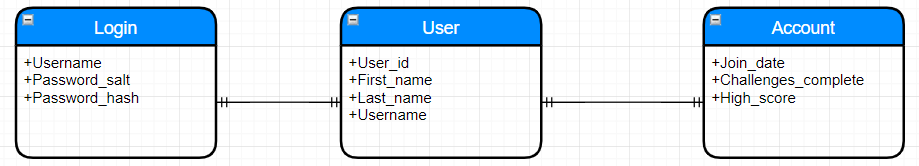
\includegraphics[width=0.75\textwidth]{Figs/User_Db.PNG} 
    \caption{User Database} 
    \label{UserDB}
\end{figure}   

\textbf{Challenges Database}   
The challenge database would be used to store each question and answer pair with a challenge Id to identify the challenge and a challenge type to group them by. The challenge database will be populated using a chosen method and will be designed later in this chapter, the idea being when the database has been populated the application could take a random challenge from the database (see Figure \ref{ChallengeDB})

\begin{figure}[!ht]
    \centering
    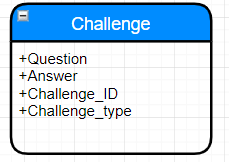
\includegraphics[width=0.25\textwidth]{Figs/Challenge_Db.PNG} 
    \caption{Challenge Database} 
    \label{ChallengeDB}
\end{figure} 

\textbf{Results Database}   
The Results Database would be used to match a user to more statistics such as total score earned, success rate, hints taken and challenges complete. This would be more used for performance analysis by teachers or supervisors to gauge the effectiveness of the application and how well certain students are performing (see Figure \ref{ResultsDB})

\begin{figure}[!ht]
    \centering
    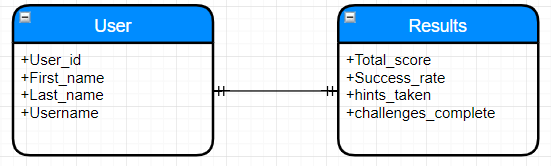
\includegraphics[width=0.5\textwidth]{Figs/Result_Db.PNG} 
    \caption{Result Database} 
    \label{ResultsDB}
\end{figure} 


%bit of research on load balancing e.g different algorithms such as random, round robin, and load based.  




\subsection{Design Methodology} 
%discuss what i am going to do pick 100 computer scientists of 3 levels of fame etc etc   
With the application theoretically designed and elements of the application discussed this dissertation will now look at how these prototyped elements will be tested and evaluated after they have been implemented to get useful data out of this project. To do this 3 different aspects of my implemented elements will be tested. 
\subsubsection{How many times does the same question come up in the same run ?} This will be testing the effectiveness of the implemented dynamic challenge generation methods and how effective each method is for randomly generating a random question. This will also answer the question of what method is superior for this intended purpose, or has the most potential for this use.  

To do this, for each script that has been made for each of the dynamic challenge generation methods, a separate version for testing that, runs through the script 100 times collecting the questions and answer pair each time then after it has ran 100 times it will look at the list of questions and answers and find how many times the same pair occurred in the run, will be made. By doing this it gives a numerical value for comparison across all of the methods and helps gauge how effective that particular method is for this chosen purpose and therefore its potential.  

\subsubsection{How many out of 100 images are faces ?}  
This test will be testing the effectiveness of the Bing API that has been chosen to use in the implementation of one of the dynamic challenge methods and for use in populating a database with challenges. By testing this it will tell us how useful this technology is and if it can be utilised for this purpose effectively. 

To test this a test case of the script will be made that uses the Bing API to collect faces for the challenge generation. In this proposed script a random topic such as 'famous computer scientists' or 'famous cryptographers' and then that is used as a search term for the Bing API which returns 100 images of that. For the purposes of this dissertation, how many of these 100 images are actually contain faces, will be tested or more accurately how many actually contain people. This will be tested by using search terms with a varying likely hood to return faces, for example,  'Famous movie stars' is very likely to return a set of actors as they by nature are well known but a search term of 'famous cryptographers' on the other hand aren't as well known by nature. Doing this will not only evaluate how useful the Bing API if for general use but analysing different topics it can also be seen how useful it is for the specific  proposed purpose 
\subsubsection{Out of 100 computer scientists, how many does the face API recognise ?} 
This will test how effective the Microsoft cognitive engine Face API, used in my proposed web scraping face quiz script, is at recognising faces. This could be a very interesting test to carry out and the data gathered from doing this would not only be useful in learning how effective it would be to use this technology for the proposed purpose but for analysing exactly how good this technology is and help determine how it is working. 

To achieve this a separate script all together will be made for this test. A list of 100 computer scientists will be gathered and separated into three levels 'world famous' e.g Bill Gates, Steve Jobs, 'industry famous' and 'well known'. Multiple images of each person on the list will then be gathered and 3 runs of each will be done of the images.Outputted will be how many of the 3 images were recognised or a 'recognition score' and how many times out of the 3 runs that API recognised the person or a 'consistency score', this will be outputted in a graphical format such as a csv file. Also featured in the tests will be  some 'dud' images of for example people who look like Steve jobs but actually are not to test how accurate the service is being. As mentioned before it is my hope that these tests will determine how useful the Face API is and help pinpoint its behaviour. 

\newpage
\section{Implementation}
After the research had been done and a theoretical design for what the application would look like and how it would work was completed it was time to start the implementation stage of this dissertation. It was then decided for the implementation to prototype certain parts of my theoretical design. The dynamic challenge generation part of the project was chosen to be prototyped as this was an important part of the learning experience to make sure that a different challenge could be given to a user each time they used the application, or if it was used in a class to ensure that all the users had different experience's using the application and couldn't copy other users answers out of laziness. Dynamic challenge generation was also an interesting area to look at and would be interesting to evaluate the effectiveness of the different approaches in creating a different challenge each time. Another part that was prototyped was the docker element of the project as docker is an incredibly useful service which would benefit the project greatly if made and prototyping an element such as database population would help illustrate that as well as gauge how efficient it would be.  

For the implementation stage Python was used for the programming language and Eclipse as the IDE. Python was chosen out of a mix of personal preference as some experience had been picked up leading up to this project and had more than any of the other programming languages as well as the practicality of using it for this project as python has extensive support libraries, useful for completing the variety of tasks that this dissertation proposed to implement, combined with the fact that it is a widely used language and recognised in the industry it seemed like a sensible choice. Eclipse was chosen to use due to exposure with it and for the purposes of this dissertation thought it better to use this rather than learn how to use a new IDE.

The Eclipse IDE will be used to develop python scripts for the different methods of dynamic challenge generation, at least a script for each. A combination of docker and python will then be used to create a service which populates a database with challenges in an efficient matter. The aim of this implementation stage is to develop something that in a later stage will give an understanding into which method of dynamic challenge generation is the most effective and how to best distribute this method.   

%include code snippets here, explain what they do etc. all scripts and docker files

%need to talk about testing strategy, how am I going to test it ? 
\subsection{Starting simple: From selection}  
\textbf{random\textunderscore selection.py}  

This script was designed to be the simplest method of dynamically generating a challenge, by just selecting from a list of question and answer pairs (see Figure \ref{Random1}) takes care of that. First off a dictionary is defined of "caesar questions" is defined, with a key and value of the question and answer. A variable of question is then defined as a random choice of that dictionary and is printed. A for loop then grabs all of answers, correct and incorrect, and prints them before reading in the users response to an answer variable. 

\begin{figure}[!ht]
    \centering
    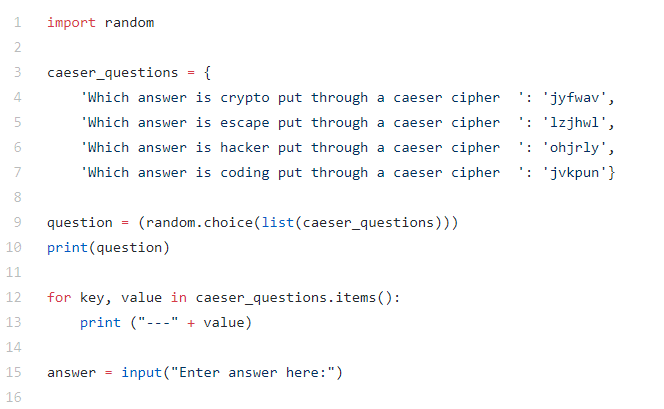
\includegraphics[width=1.0\textwidth]{Figs/random1.PNG} 
    \caption{Question selection} 
    \label{Random1}
\end{figure}   

A function is then defined that loops through all of the items in "caesar questions" and compares the answer given by the user to the answer pair to all of the questions. If a match is found then the value "correctAnswers" is set to the corresponding question to the answer given, otherwise it remains empty. Finally the "answerChecked" value is set to what has been returned by that function, if this is equal to the question given at the start "correct" is printed if not "incorrect" is printed (see Figure \ref{Random2}).

\begin{figure}[!ht]
    \centering
    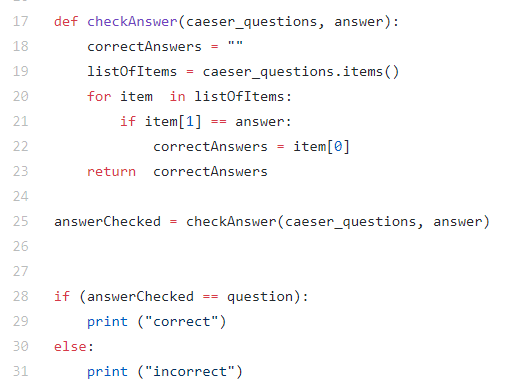
\includegraphics[width=1.0\textwidth]{Figs/random2.PNG} 
    \caption{Answer Check} 
    \label{Random2}
\end{figure} 


\subsection{Using API request}   

This script was created to implement the API method of dynamic challenge generation. In practice it would be more useful to do this with an actual website or service designed for this use but for test purposes a script to represent the API being called to for the answers was made.  

\textbf{API.py}    

First the API that was to be called for a question was implemented. An API that when ran would run on local host using python Flask was set up. A route for the request to be sent and read in a string that will represent the question to be sent back, was then set. depending on the value of the question string the API selects a question answer pair and returns it (see Figure \ref{API}).


\begin{figure}[!ht]
    \centering
    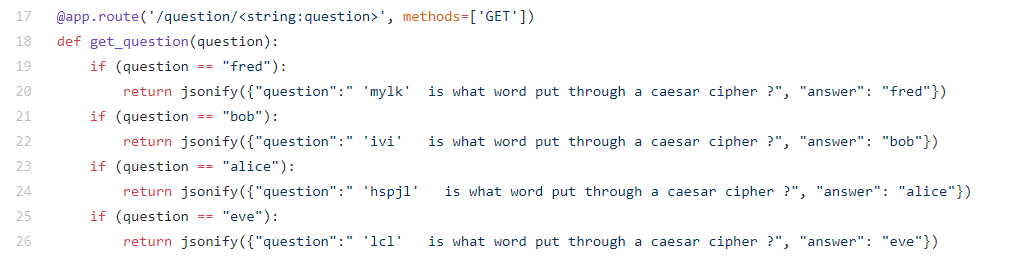
\includegraphics[width=1.0\textwidth]{Figs/API.PNG} 
    \caption{API} 
    \label{API}
\end{figure}

\textbf{API\textunderscore request.py} 
Next up a script that would make a call to this API to get a question shown in (see Figure \ref{API request}) was implemented. First off a set of tags to be sent are defined in "questions" and "question" is set to a random choice of them. a GET request is then sent to the API and the response is read in, each value contained within the json response is also read into "values". the "user question" and "user answer" variables are set to the question contained in the response and the answer contained in the response respectively, the question is then is then asked to the user and their answer compared to the answer. 

\begin{figure}[!ht]
    \centering
    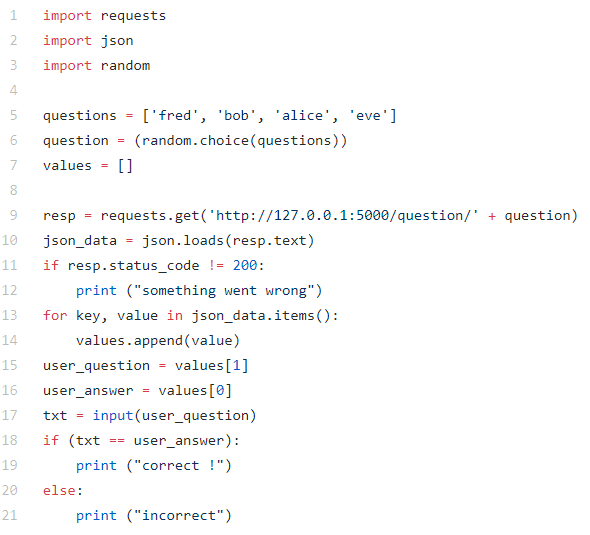
\includegraphics[width=1.0\textwidth]{Figs/API request.PNG} 
    \caption{API Request} 
    \label{API request}
\end{figure}

\subsection{Web scraping} 
\subsubsection{Basic web scraping}   
For my more basic attempt at a web scarper a basic website was found listing off "30 influential computer scientists" and used it to pick them off and use them to generate questions. a hard coded hash method is shown and then a method of opening an online hash generator and putting the text through that as well. 

\textbf{Web\textunderscore scraper\textunderscore final.py}  
For this web scraping application the BeautifulSoup library was used for the opening of the website and getting names and the selenium library for opening open a browser and putting the text through an online hash generator. First off (see Figure \ref{Webscrape1}) the source was set to the website that was chosen to be used and defined an empty list "people". Then the content returned from the web page is taken and sifted through to find what is wanted. The web page is inspected and the headers were found that contained the information that was wanted to be picked out (the names) so the data returned from the source was split accordingly. After the text was almost down to the strings that were wanted it was filtered further and appended the filtered string to a list of people before "popping" some excess items that came after the desired list of people. A random "person" is selected from the list of "people" found from the website and after this a SHA256 hash is generated of the person from the list and displayed. 

\begin{figure}[!ht]
    \centering
    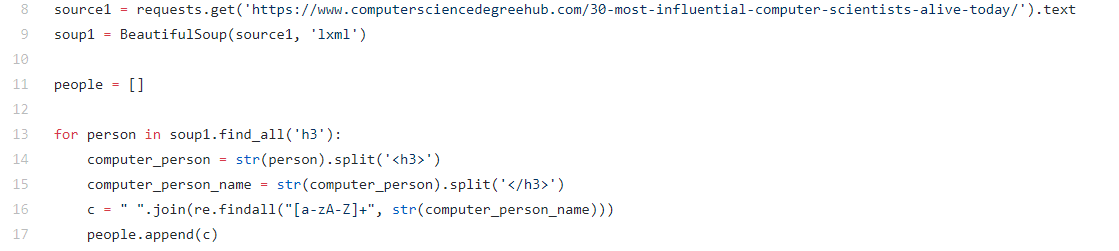
\includegraphics[width=1.0\textwidth]{Figs/web_scrape1.PNG} 
    \caption{Web scraping the names} 
    \label{Webscrape1}
\end{figure}  

 A web page that calculates md5 hashes of a value that is typed in is opened (see Figure \ref{Webscrape2}). By inspecting the web page the elements needed were identified such as the text box to enter the value to be hashed, which was set as "hashField", also identified was the area which the calculated hash is displayed and set that as "hashResult". The "person" that was chosen was sent to the text field "hashField" and once the value was entered read the value of what was in the returned hash field to "hashResult". This value was then printed along with the original person.

\begin{figure}[!ht]
    \centering
    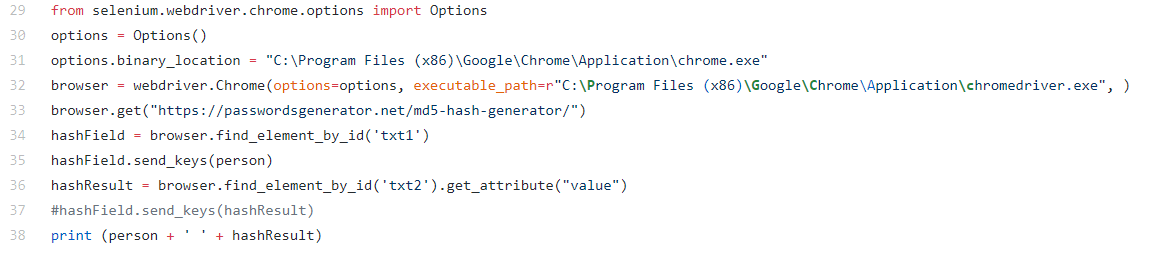
\includegraphics[width=1.0\textwidth]{Figs/web_scrape2.PNG} 
    \caption{Getting hash through browser} 
    \label{Webscrape2}
\end{figure} 



\subsubsection{Web scraping with facial recognition}   

For this approach the services of Microsoft Azure were taken advantage of using two API services available from from their cognitive services. The Bing search API and the Computer Vision API which uses the Microsoft cognitive engine. Both were set up on a Microsoft Azure account that was created (see Figure \ref{Azure}) and used them to generate the keys and the links that were needed to make my API calls in the script. This script will use the Bing search API to find 100 images of a search term then use the Vision API to recognize a face contained in an image from the search, if it matches a face to the name then it displays to user and asks who they are. 

\begin{figure}[!ht]
    \centering
    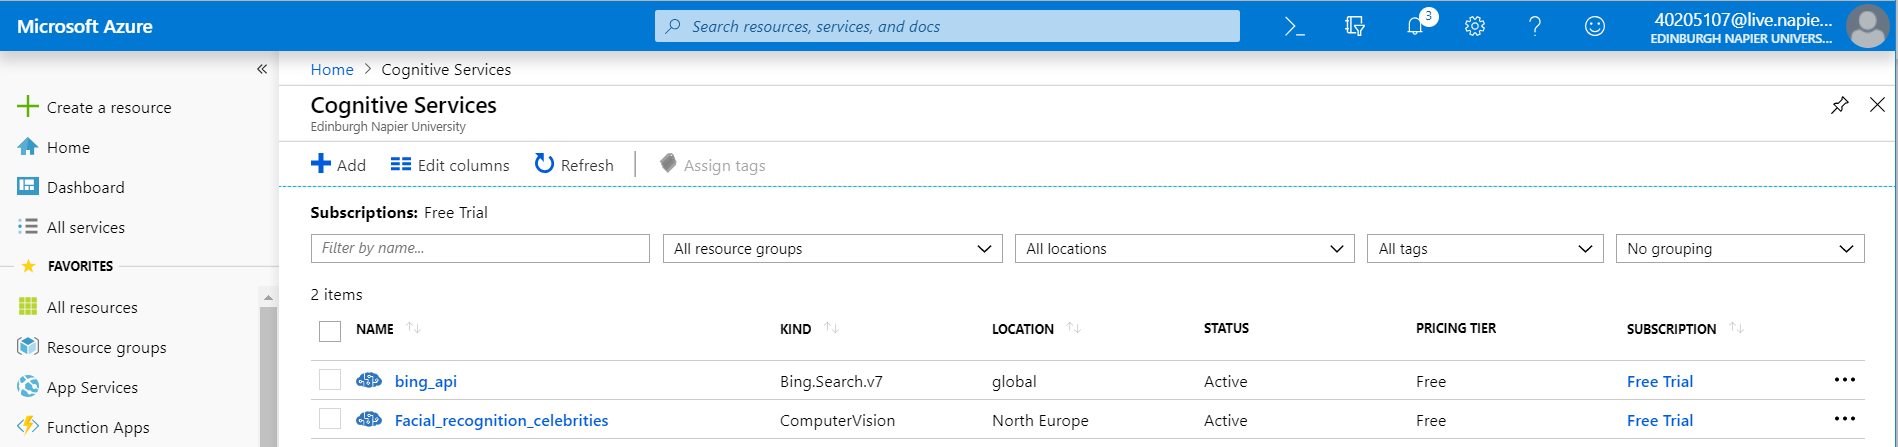
\includegraphics[width=1.0\textwidth]{Figs/Azure.PNG} 
    \caption{Microsoft Azure Cognitive Services} 
    \label{Azure}
\end{figure}

\textbf{Face\textunderscore quiz\textunderscore final.py} 

At the start of the script variables are declared such as a list of random cyber security topics to be chosen from such as "famous computer scientists" or "famous cryptographers" , a search term to be used for the Bing API which is a random choice of those topics and other variables used for the APIs such as subscription keys and headers and params etc. Then the findImages function is defined (see Figure \ref{findimages}). In this function the API client is set up using the credentials set, then call the API with the search term decided and a count of 100 set as well as a filter of face applied. A random image is then chosen and  the image url is returned. 

\begin{figure}[!ht]
    \centering
    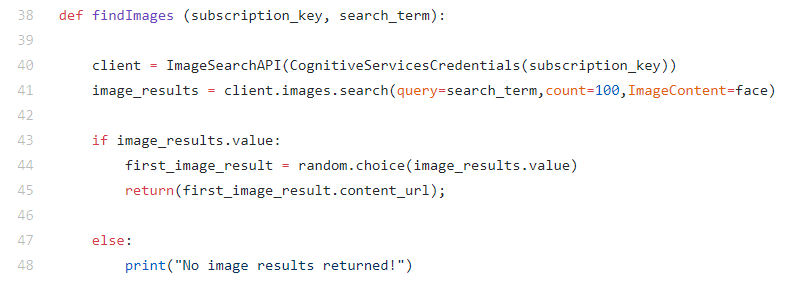
\includegraphics[width=1.0\textwidth]{Figs/findimages.PNG} 
    \caption{findImages function} 
    \label{findimages}
\end{figure}  

Next up the findMatch function was defined (see Figures \ref{findmatch1} \ref{findmatch2}). First the search term to be used within the function is declared and the findImages function is called with that search term, which as discussed, returns an image url that is concatenated in the "body" variable used to send a request to the vision API. The connection to the vision API is set up and a request is sent using that image url as the body. What gets returned is a json response which is broken down into data and is used in the next part to determine whether a match has been found or not. This is done handling certain errors which would mean a match has not been found. Multiple runs were done and caught the different errors that were happening if a match wasn't found. For example if the categories or celebrities bracket was empty it meant that there was no match found for the face and when a name value was attempted to be read in and error would happen, with these errors that mean no match had been found the string "no match" is returned at their occurrence. Other exceptions to note was sometimes a match is found but when the image url was trying be accessed the website denied permission and sometimes it would return an image of multiple people which obviously isn't helpful when trying to ask a user who they are as it could be confusing as to which person the question would be referring to, this was solved by accessing the classification parameter and only accepting pictures that were wither of a person or a portrait of a person (dropping images classified as group images). These exceptions were handled and also returned "no match" if they occurred. If none of these exceptions occur then it means a match has been found and a name has been able to be matched to the face so the image url is returned.

\begin{figure}
\centering
\begin{minipage}{.5\textwidth}
  \centering
  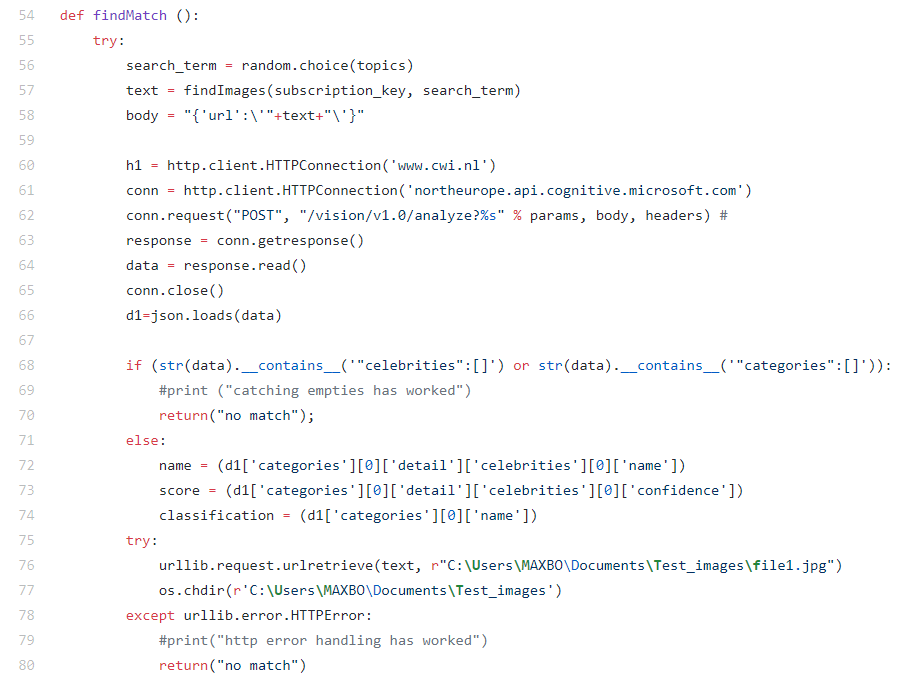
\includegraphics[width=1\linewidth]{Figs/findmatch1.PNG}
  \captionof{figure}{findMatch function pt 1}
  \label{findmatch1}
\end{minipage}%
\begin{minipage}{.5\textwidth}
  \centering
  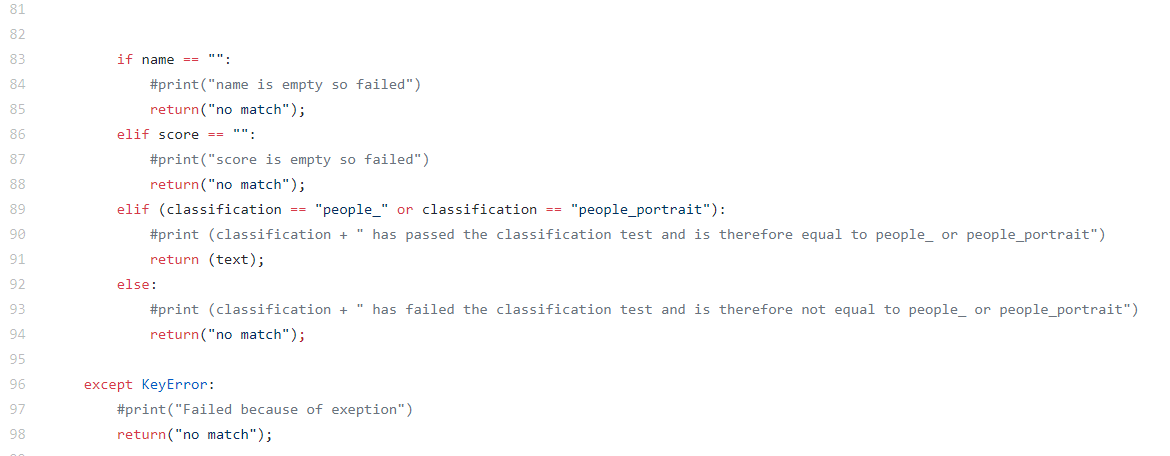
\includegraphics[width=1\linewidth]{Figs/findmatch2.PNG}
  \captionof{figure}{findMatch function pt 2}
  \label{findmatch2}
\end{minipage}
\end{figure}   

After this the getAnswer function is defined (see Figure \ref{getAnswer}). Firstly the vision API was et up to be used for the question, then sends an image to it, the vision API responds and the name is taken from the response and stored in a variable "name", the certainty score is also taken and rounded up and stored in a variable. Then the image is opened and the user is asked who it is, if they're answer matches the name determined from the API "correct" is returned if not "incorrect" is returned. 

\begin{figure}[!ht]
    \centering
    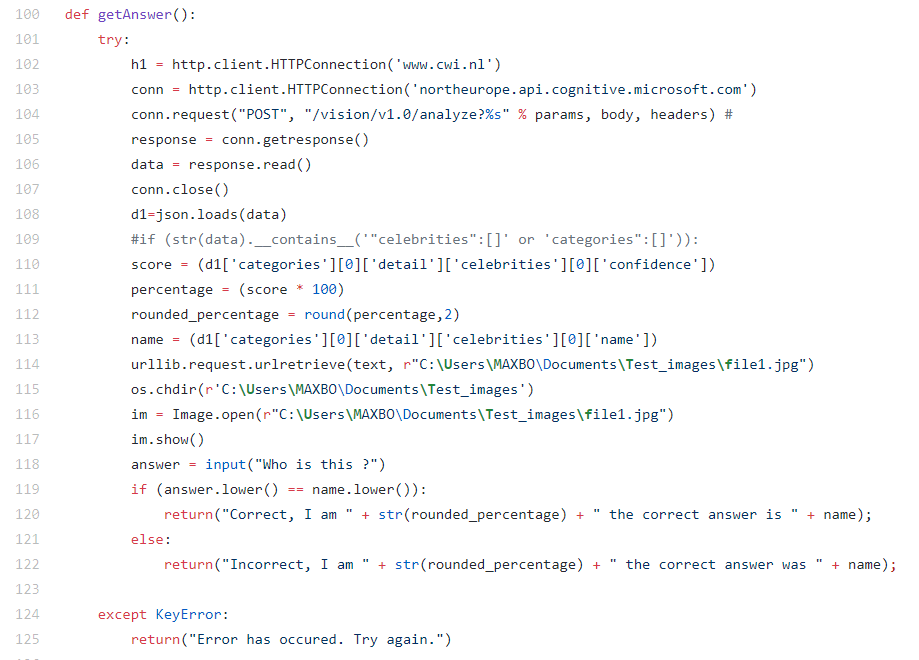
\includegraphics[width=1.0\textwidth]{Figs/getanswer.PNG} 
    \caption{getAnswer function} 
    \label{getAnswer}
\end{figure}  

A variable of correct answers is set to 0. The finally inside a for loop that iterates 5 times, is a while loop that calls the findMatch function setting the variable "text" to the value it returns. The while loop breaks when the value returned is not equal to "no match", so essentially, if the image has not triggered any of the exception and a name has been mapped to the face, when this happens "text" is set to the image url and the while loop is broken. The "body" variable is then defined with that image url and the getAnswer function is called asking the user who is in the image and determining if they are correct. If the function returns correct answer then the correct answer variable is incremented by 1. After this process has been iterated through 5 times a score out of 5 is given and the script terminates (see Figure \ref{askquestion}).

\begin{figure}[!ht]
    \centering
    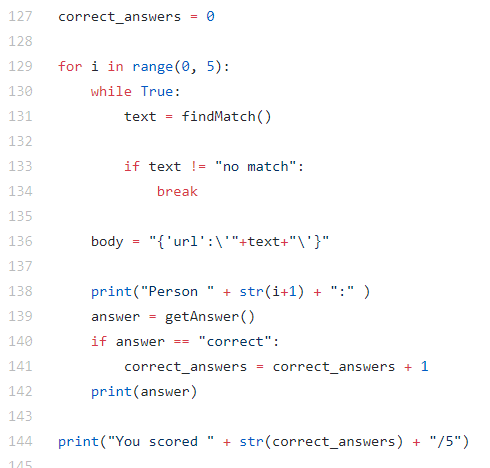
\includegraphics[width=1.0\textwidth]{Figs/askquestion.PNG} 
    \caption{Asks user question and iterates} 
    \label{askquestion}
\end{figure} 




\subsection{Challenge distribution with Docker} 
\subsubsection{Python}   
This python script was adapted from the face quiz script but with the use of the pymongo library used to insert challenge data into a MongoDb database. 

\textbf{"Docker\textunderscore face\textunderscore pop\textunderscore final.py"}   

The Docker face population script is very similar to the Face Quiz script discussed in the previous section. The only difference is that it doesn't have the getAnswer function as there is no user interaction and is therefore unnecessary to ask the user the questions and iterate through the process 5 times at the end. The other difference is the use of the pymongo library which is used to when the findMatch function determines there has been a match on the face, takes the "question" that would be asked, the image url for the selected image and the "name" of the person in the image (or the answer) and inserts it into the challenge Database (see Figure \ref{dbinsert2}). In the code (see Figure \ref{dbinsert1}) the "db" referred to as the host on line 43 is established in the docker compose file and is discussed later.  .

\begin{figure}[!ht]
    \centering
    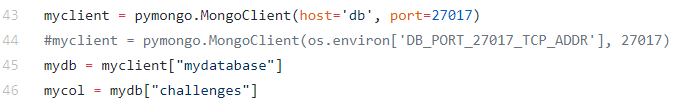
\includegraphics[width=1.0\textwidth]{Figs/dbinsert1.PNG} 
    \caption{Establishing Database connection} 
    \label{dbinsert1}
\end{figure}  

\begin{figure}[!ht]
    \centering
    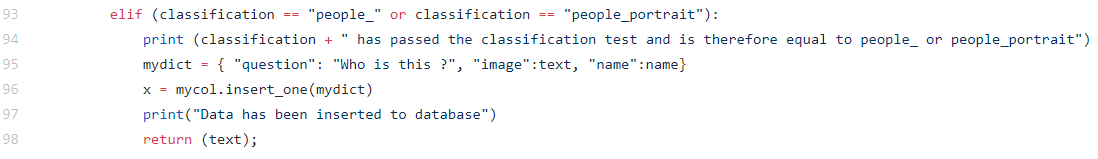
\includegraphics[width=1.0\textwidth]{Figs/dbinsert2.PNG} 
    \caption{Inserting data into the database} 
    \label{dbinsert2}
\end{figure} 

\subsubsection{Docker}   
These are the files used to create Docker images and spin up the containers with my script running inside them so the database can be populated. 
\textbf{requirements.txt}   
This file is essentially just a list of all the external libraries used in the script that the machine will be running. The Dockerfile uses this file to pip install everything to contained inside (see Figure \ref{req}) 

\begin{figure}[!ht]
    \centering
    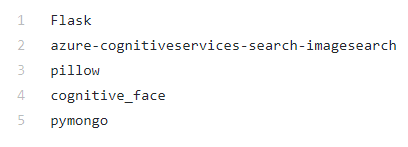
\includegraphics[width=1.0\textwidth]{Figs/requirements.PNG} 
    \caption{Requirements.txt contents} 
    \label{req}
\end{figure} 

\textbf{Dockerfile} 
The Dockerfile its the instructions that are needed to build the docker image that will be spinned up in containers.  This included installing the requirements (as discussed in the previous section), copying the python script (docker\textunderscore face\textunderscore pop.py), exposing the port so it can contact the database and finally running (see Figure \ref{Dockerfile}). 

\begin{figure}[!ht]
    \centering
    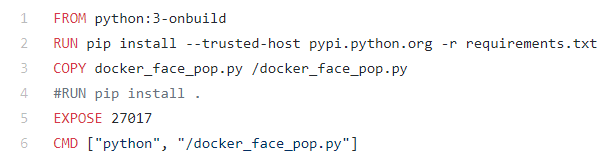
\includegraphics[width=1.0\textwidth]{Figs/Dockerfile.PNG} 
    \caption{Dockerfile contents} 
    \label{Dockerfile}
\end{figure}  

\textbf{docker-compose.yml} 

Docker compose is a tool for defining and running multi container applications which can be used to configure the application. After this has been done all services can be created and started with a single command. Docker compose was used to establish the services of "db" (this is the db reffered to in the docker face population script) which is a mongoDB image that was downloaded off of Docker Hub (where you can download from a library of images) and expose the correct ports and set the volume. Then the "client" is defined as using honours-project image (the image created using my requirements.txt and Dockerfile) and link it to the db service so data from the client service can be inserted into the database from the db service. The port is opened and then the environment that will be worked with (which database is going to be used etc) is established.

\newpage
\section{Results and Evaluation} 
%Results for for tests:out of X runs how many times did the same question show up ? to evaluate the three dynamic challenge generation method. test how many faces show up in search out of 100 ? to evaluate bing API effectiveness for different topics such as computer scientists and cryptographers. Out of 100 faces how many correct ? to evaluate facial recognition. Then evaluate further effectiveness of facial recognition by taking 100 famous computer scientists, cryptographers etc of varying fame level, very famous to kind of famous to not very famous and test success rate. feed it some duds, Bill Gates look a like etc.  
\subsection{Test 1: how many times does the same question come up in the same run ?}  
\subsubsection{Making the test cases} 
To perform this test on the different dynamic challenge methods altercations were made to the code of each of the methods so it would return the data wanted for the purposes of this test and this dissertation (see Figure \ref{testcases}) this particular example is taken from the random selection method but the code added to them all was pretty similar, just minor changes depending on how the questions were generated in each of them. These changes consisted of making a list "questions" which each question is added to as the script iterates though the process, "unique\textunderscore question" is another list declared which will be added to every time a question appears and hasn't yet been appended to "questions" (if this is the first time the question appears and is therefore unique). "occurrence \textunderscore count" is added to every time a question is retrieved that is in "questions" and therefore has already been asked. it then iterates through the question asking process 100 times. After this "ocount" is declared which is used to add the total number of occurrences for each unique question, this is used at the end of the script to calculate the average occurrence of a question in 100 runs. Also printed out is how many times each question showed up in that run and how many appearances of the same question there was in that run (see Figure \ref{exout1}).

\begin{figure}[!ht]
    \centering
    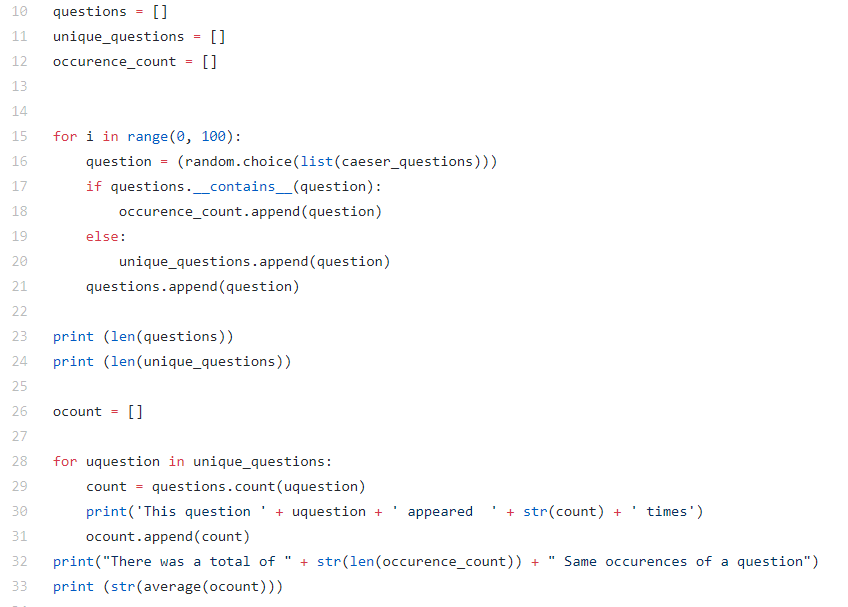
\includegraphics[width=1.0\textwidth]{Figs/testcases.PNG} 
    \caption{Example of changes made to produce test results} 
    \label{testcases}
\end{figure} 

\begin{figure}[!ht]
    \centering
    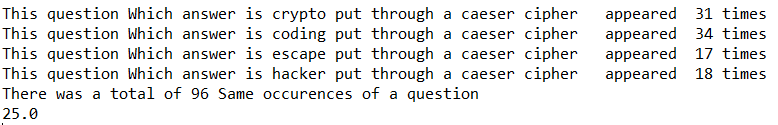
\includegraphics[width=1.0\textwidth]{Figs/exampleoutput1.PNG} 
    \caption{Example output of test cases} 
    \label{exout1}
\end{figure}  

\subsubsection{The Results} 
First data was collected and a graph was made illustrating the average question occurrence in 100 runs. So for each of the unique questions asked how many times on average was it asked across the 100 runs (see Figure \ref{r1}). The Random selection and API request was 25 times, web scraping was 3.44 times and web scraping with web scraping with API was 1.51 times.

\begin{figure}[!ht]
    \centering
    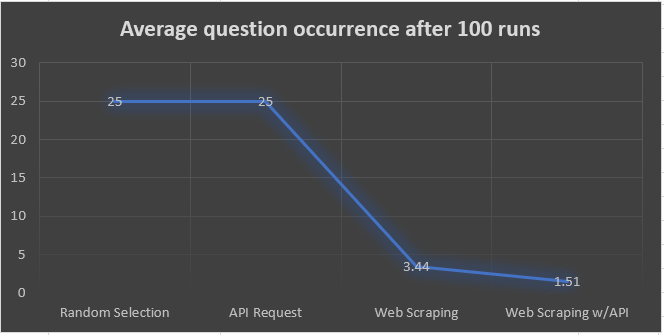
\includegraphics[width=1.0\textwidth]{Figs/results1.PNG} 
    \caption{Average Question Occurrence} 
    \label{r1}
\end{figure} 

Next the number of times that a question that had already been asked was asked was taken for each of the methods (see Figure \ref{r2}). Random selection and API request methods had 96 occurrences of the same question, the web scraping method had 71 and the web scraping method using APIs had 34.

\begin{figure}[!ht]
    \centering
    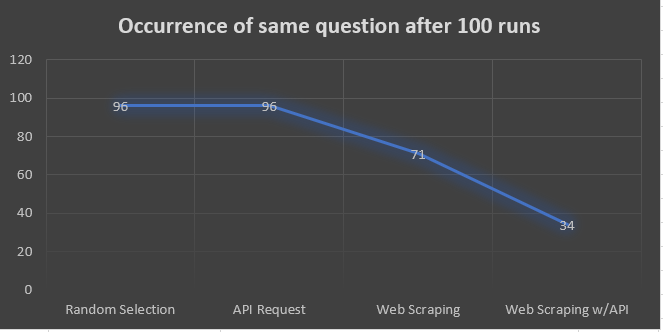
\includegraphics[width=1.0\textwidth]{Figs/results2.PNG} 
    \caption{Same Question Occurrence} 
    \label{r2}
\end{figure}  

Finally both of the results previous tests were taken plotted on a graph  (see Figure \ref{r3}) to show the correlation.

\begin{figure}[!ht]
    \centering
    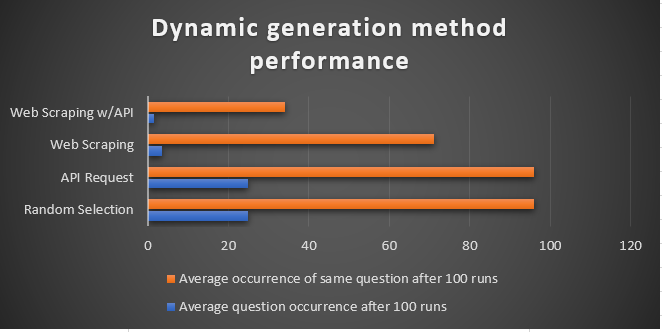
\includegraphics[width=1.0\textwidth]{Figs/results3.PNG} 
    \caption{Dynamic Generation Method Results Correlation} 
    \label{r3}
\end{figure}  

\subsubsection{Evaluation of Results} 

Test 1 was evaluating the performance of the different methods of dynamic challenge generation. When discussing these results and the ones soon to follow it is important to acknowledge that the implementation of both the API request and random selection methods were both very simple. With a selection of 4 questions to choose from the performance was never going to be very high when it comes to dynamic challenge generation. Adding another question to the selection would slightly increase the the performance and so on and so on. This could go on forever but for these methods would require a lot of hard work and hard coding in potential challenges. So when looking at these numbers instead of evaluating these results for these specific scripts it should be evaluated as the potential this method carries to be scaled for the intended use based on the results received.  

The first set of data collected was how many times on average, per unique question, did it show up in 100 runs. Random selection and API request methods both had 25 whereas web scraping only had 3.44 and web scraping with the use of API had 1.51 times, meaning that in 100 runs the average question only came up 1.51 times. This is significantly better than both the API request and random selection methods and over 2x better than the web scraping method. These results show that the web scraping with API method has a lot more potential and has a proclivity to generate a new unseen question, more so than any of the other methods. 

The second set of data collected showed how many times in 100 runs did an occurrence of the same question happen. Random Selection and API request methods both had 96 occurrences of the same question, web scraping had 71 and Web scraping with API had 34. Again web scraping with API method is in front out performing all of the other methods of dynamic challenge generation. With 34 same occurrences of the same question in 100 runs that means 66 unique challenges were generated in 100 runs (29 for web scraping and 4 for random selection and API request) this is an impressive number and shows the potential this method has. 

Overall this test has shown that the use of the web scraping with API method has more potential for the use of dynamic challenge generation with it out performing the other 3 by quite a bit. As discussed the implementation of this should be considered but even if more challenges were added to the first two methods you would have to add a lot and it would take a lot of time to achieve the same sort of numbers being returned from web scraping with API. Web scraping as a method as a whole has great potential and is superior both to random selection and API request methods for this purpose, however the use of APIs to aide this method gives it an edge and increases the performance. The APIs also do a lot of the heavy lifting in that they return images, or facial matches and you don't have to manually mine the elements you need as with web scraping on its own.

\subsection{Test 2: How many faces out of 100 images ?}.   
\subsubsection{Making the test case}
For this test a test script was made which called the Bing API and asked for 100 images with the face tag with four different search terms - "famous people", "famous actors", "famous computer scientists" and "famous cryptographers". The idea being to test the Bing APIs ability to accurately and consistently produce pictures of faces, using different search terms increasing in specificity to gauge how this affects it. A test case script was made for the evaluation of this simply taking a search term and calling the Bing API to return one hundred images with the face tag. The selenium library was then used to iterate through the content url of each of the 100 images returned and open them in a browser. This allowed me to quickly scan through the images looking for ones that did not contain a face. This was done for each search term changing the variable "search\textunderscore term" accordingly each time (see Figure \ref{bingevc}).  

\begin{figure}[!ht]
    \centering
    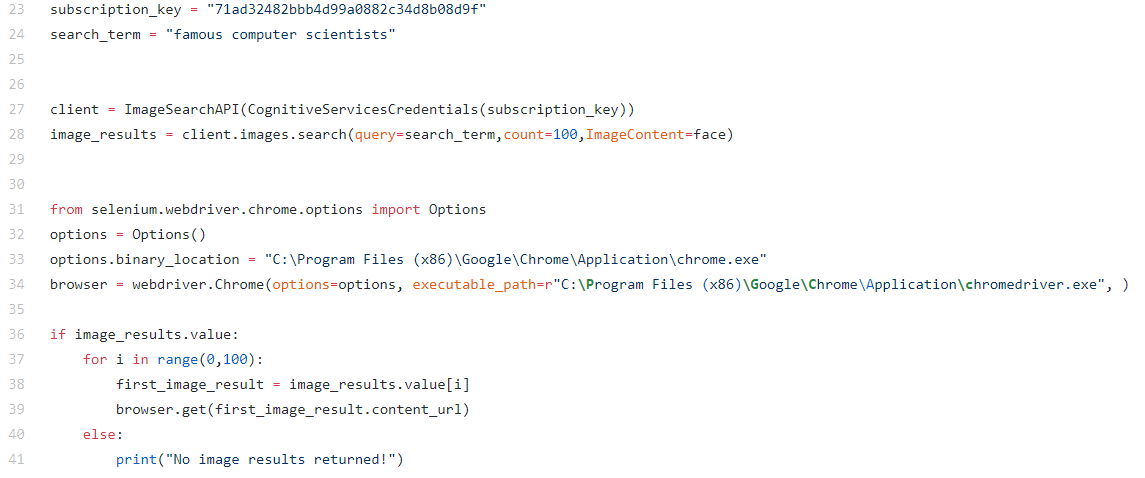
\includegraphics[width=1.0\textwidth]{Figs/bingevcode.PNG} 
    \caption{Code used for Bing API test case} 
    \label{bingevc}
\end{figure} 

\subsubsection{The Results} 

The results were collected and each occurrence of "non face"  images in the 100 returned by the Bing API was counted for each search term 3 times to ensure accurate results.Both the "famous people" and "famous movie stars" returned 100 out of 100 images containing faces. "famous computer scientists" returned 93 out of 100 images containing faces and "famous cryptographers" returned 37 out of 100 images containing faces (see Figure \ref{bingev}). 


\begin{figure}[!ht]
    \centering
    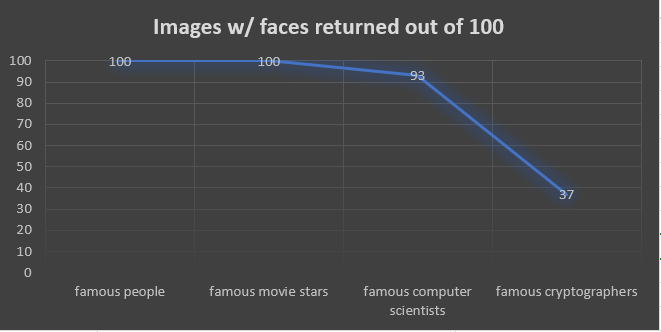
\includegraphics[width=1.0\textwidth]{Figs/bingev.PNG} 
    \caption{Bing API performance} 
    \label{bingev}
\end{figure}

\subsubsection{Evaluation of Results} 

Test 2 was evaluating the performance of the Bing API used in the implementation of my web scraping with API dynamic challenge generation method. The Bing API has a query parameter called ImageContent which you can use to specify you want faces to be returned, this was done for all the runs.

The data collected for this test was measuring how many images out of the 100 that were returned, contained faces (and therefore could be used for the intended purpose more effectively). This was done using four different search terms "famous people", "famous movie stars", "famous computer scientists" and "famous cryptographers" as discussed in the results chapter the idea was to gauge how effective the Bing API was at returning faces the more specific the search term got, with "famous people" and "famous movie stars" likely to return very well known people and "famous computer scientists" and "famous cryptographers" with being more specific search terms they have less possibilities to collect from, this is important to evaluate as with the intended purpose these specific search terms would be getting used.  

The "famous people" search term returned 100 out of 100 images containing faces, as did "famous movie stars", "famous computer scientists" returned 93 out of 100 images containing faces and "famous cryptographers" only returned 37 out of 100 images containing faces. This shows a dramatic decrease in the amount of images containing faces returned when the search term gets as specific as "famous cryptographers". The images returned were of graphs explaining cryptography terms, pictures of books, pictures of keys etc essentially things that are associated with cryptography but not actually famous cryptographers a lot of the time. From context it seems this is because that there are less big names associated with cryptography, at least in the same manor as the other search terms, and so the results that Bing collects the images from are discussing cryptography rather than a person associated with cryptography so return these images. This isn't a massive blow to using the Bing API for the intended purpose, as has been shown it can still be effective and if you use a variety of search terms with varying specificity as this dissertation has it stops the challenge generation from relying on this specific search term. However it is important to note that the more specific the search term the less option it has to choose from for faces and therefore will take longer to return a face that has been matched and therefor if this search term is used soley will likely slow down the process. 

\subsection{Test 3: Out of 100 computer scientists, how many does the face API recognise ?}  

\subsubsection{Making the test case}

To make the test case for the face API evaluation alterations were made to the face quiz application. The first step however to select a list of 100 computer scientists. 100 names were gathered and grouped them by fame level. 10 very famous 15 well known and 75 industry recognised, this list is available in the appendix. After this list was decided the alteration was started by declaring three dictionaries, one for each fame bracket. In this dictionary was three image links for each person in the list, which was sourced independently rather than using the Bing API previously used in the project to ensure the data was consistent, in that they were a similar quality of photo, and accurate, in that the images were of who they were supposed to be. Other changes included adding two functions one similar to the findMatch function used earlier except it returned the certainty score called getScore and a second which just took the digits off of the end of the names of the people (as they were numbered 1-3 so that they were different keys) called mySplit. Then for each of the three dictionaries the following was done: Three variables were declared; “xcorrect” to count how many correct matches, “xscores” to collect the certainty scores of the matched faces and finally “xmatched” which collects the names of all of the people that have been matched. Then a for loop iterates through each of the values in the dictionary trying to find a match to the face, appending to the lists and incriminating the correct counter when a match is made  (see Figures \ref{fec1} \ref{fec2} \ref{fec3}).  After this has been done for all three dictionaries, the results are displayed giving: how many celebrities in that category were matched, the average confidence rating given with matches for that category and the total pictures that were matched (see Figure \ref{feo}).    

\begin{figure}[!ht]
    \centering
    \includegraphics[width=1.0\textwidth]{Figs/faceevalcode1.PNG} 
    \caption{Setting up of dictionaries} 
    \label{fec1}
\end{figure} 

\begin{figure}[!ht]
    \centering
    \includegraphics[width=1.0\textwidth]{Figs/faceevalcode2.PNG} 
    \caption{Appending lists and incriminating count} 
    \label{fec2}
\end{figure} 

\begin{figure}[!ht]
    \centering
    \includegraphics[width=1.0\textwidth]{Figs/faceevalcode3.PNG} 
    \caption{Formatting data to be output} 
    \label{fec3}
\end{figure} 

\begin{figure}[!ht]
    \centering
    \includegraphics[width=1.0\textwidth]{Figs/faceevaloutput.PNG} 
    \caption{Example output of Face API test case} 
    \label{feo}
\end{figure} 


\subsubsection{The Results}

For this test fed the Face API 3 different pictures of each of the computer scientists, and did three runs of the script and averaged out the results. The first metric measured was how many people were recognised, the average was 10 out of 10 for the very famous category, 15 out of 15 for the well known category and 58 out of 75 for the industry recognised (see Figure \ref{fer1}). This equates to a total of 83 out of 100 computer scientists being recognised. 

\begin{figure}[!ht]
    \centering
    \includegraphics[width=1.0\textwidth]{Figs/faceevalr1.PNG} 
    \caption{Face API people recognised} 
    \label{fer1}
\end{figure}

For the next part of this test the average picture recognition was measured, meaning the face API might have recognised the computer scientist but how many of the 3 pictures did it recognise ? Essentially how consistent was the Face API across all the 3 fame categories. The averages were 27 out of a possible 30 images recognised for the very famous category, 36 out of a possible 45 images were recognised in the well known category and 120.6 out of a possible 225 images were recognised in the industry recognised category, on average (see Figure \ref{fer2})  

\begin{figure}[!ht]
    \centering
    \includegraphics[width=1.0\textwidth]{Figs/faceevalr2.PNG} 
    \caption{Face API images recognised} 
    \label{fer2}
\end{figure}

The third and final metric gathered was the average confidence rate of the matches made, the Face API gives a confidence rating along with the match stating how sure it is that it is that person. The average confidence rating for the very famous category was 99.43 percent, the average confidence rating for the well known category was 98.54 percent and the average confidence rating for the industry recognised category was 98.71 percent (see Figure \ref{fer3}). 

\begin{figure}[!ht]
    \centering
    \includegraphics[width=1.0\textwidth]{Figs/faceevalr3.PNG} 
    \caption{Face API average confidence ratings} 
    \label{fer3}
\end{figure} 

All of these results were then taken and mapped on a graph to show a correlation (see Figure \ref{fer4}) 

\begin{figure}[!ht]
    \centering
    \includegraphics[width=1.0\textwidth]{Figs/faceevalr4.PNG} 
    \caption{Face API performance} 
    \label{fer4}
\end{figure} 

\subsubsection{Evaluation of Results} 
Test 3 was evaluating the performance of the Face API used in the implementation of my web scraping with API dynamic challenge generation method. 
As previously mentioned for this test a list of 100 computer scientists was made and separated them into different fame categories to try and see how effective the Face API was in determining each different category. The first set of data collected for this test was how many people in each category were recognised. In both the very famous and well known categories all of the computer scientists were recognised where as with the industry recognised category 58 out of 75 were recognised, resulting in a total of 83 out of 100 computer scientists recognised. This performance was as expected in that the recognition rate of the people was less as they became less known however this performance was still relatively high. Even with 75 people included that were not very famous the Face API still managed to recognise over 80 percent of the 100 people.  

The next set of data collected was how many of the actual images were recognised. Here this dissertation was investigating although the Face API may have recognised one of the images of the computer scientist, How consistent was it across the 3 images provided. The scores came back as follows: 27 out of 30 images recognised for the very famous category, 36 out of 45 for well known and 120.6 out 225 for industry recognised. This equates also to 2.7 out of the 3 images provided on average for very famous, 2.4 out of 3 for well known and 1.6 out of 3 for industry recognised. Here we see a more drastic drop in performance when it comes to the lesser known people, although the Face API was able to recognise over 77 percent of the people included in the industry recognised category it only recognised 53.6 percent of the total images in the same category. this is quite a drastic drop and should be taken into account for this considered purpose. This would suggest maybe it best to gather multiple images of people if intending to use them, if they are lesser known as this could be down to the API learning who certain pictures are but struggling to match them when a face is at a different angle.  

The final set of data collected was the average certainty rating given when a match was made. The results were fairly consistent through out all of the categories with very famous having 99.43 percent, well known having 98.54 percent and industry recognised having 98.71 percent. While it can be seen that technically the industry recognised category has a marginally higher average confidence rating but this is likely insignificant and the point to take from these results is that the confidence ratings returned from the Face API are very high, and consistently very high which is essential if its to be used for this intended purpose. 

Overall the Results show that the Face API is very effective with it recognising 83 out of 100 computer and the average confidence rating being over 98 percent in all three categories, the only area of concern is the rate at which it recognises images in the lesser known category with almost half of the images not being matched. This is not as much of a problem as this can be balances out by feeding multiple images of the same person to find a match. Analysing the performance of this API it can definitely be deemed effective and suitable for the intended use.  

\subsection{Evaluation of Results as a whole} 

Overall the implementation stage has proved effective in determining the dynamic challenge generation method with the most potential is web scraping with API. The Bing API proved effective but the performance got gradually worse the more specific the search term got, as discussed this isn't fatal but should be considered when using the Bing API for generating cyber security challenges, as proposed. The Face API performed well in the tests provided also with a high recognition rate and the low photo recognition for the lower fame tier being an issue that is easily remedied by supplying a surplus of images this API can be deemed suitable for this purpose and furthermore can give an edge in challenge generation that wouldn't be possible without. 


\newpage
\section{conclusions} 
\subsection{Summary of conclusions}
A review of the literature was done, investigating different learning model, their significance and use in the classroom and more specifically their use in computer science. After this the literature on CTF learning was reviewed before finally taking a more in depth look at the literature on gamification which showed the various uses and the potential it has for cyber security education (as well as various pitfalls to avoid), furthermore suggesting that there maybe be a way to combine gamification and learning models such as Blooms taxonomy. This knowledge was then taken and applied to a theoretical design for an application that would teach young audiences cyber security before technical elements behind the application were discussed, including dynamic challenge generation methods, which were designed and implemented. After the implementation, test case scripts were made in order to evaluate the performance of the methods and the APIs utilised. The results fed back suggested: Web scraping with the use of APIs is the most effective method of dynamic challenge generation, and that both of the APIs used, while the performance slightly suffer from the specificity  that comes with certain areas of cyber security, have impressive performance results that justify their use for this purpose.

\subsection{Achievement of aim and Objectives}  
In this section this dissertation will discuss how well this project has met the aims and objectives set at the beginning of the project.  

The first aim of this project was to do the relevant research looking into different learning techniques and further into CTF learning to provide a literature review. This project succeeded to meet this aim, the literature was well researched and covered all of the areas of identified interest, as well as learning models and CTF learning, extensive research was also done on gamification and how this could be applied to the classroom. Ultimately the aim was to cover the topic to a point where an application with the intended purpose of engaging a younger audience with cyber security in answer to the cyber security skills gap could be proposed and designed, the literature review in chapter 2 of this dissertation met this aim.   

The second aim of this project was to take what was learned from the literature an use it to design a proof of concept for an application that took into account the literature discussed. The design chapter of this project achieved this aim, this dissertation took what was learned about learning models and gamified learning as well as aspects of CTF styled learning and applied these to design the architecture of how this application would work, mocking up how it would look and technically designing aspects of it that would later be implemented. 

The first objective was designing the application with reference to the literature which as just discussed was achieved. The next step was to design learning materials to be used in conjunction with the application, it was originally intended to mock up about 5 lessons to give a wider span of what the application would look like however due to time it was decided to mock up 3 and concentrate on them. The next two objectives were to design technical aspects of the proposed application and implement them, the first of which being completed in the technical design sub chapter and the second of which being completed in the implementation chapter. With more time more detail would have went into the technical design of the application and maybe how the application could have been built as a web application, how that would have been structured and how it could have been scaled would have been discussed and included in this dissertation but also due to time constraints sound attempt could not have been delivered. The final objective was to test and evaluate the useful of the prototype elements, this was a success, this dissertation performed a series of appropriate tests that collected interesting data allowing for it to come to the conclusions that were desired without ambiguity.  

Overall, although some sacrifices were made due to time, this dissertation has satisfied for the most part all of the aims and objectives set at the beginning and that this project achieved what it set out to.

\subsection{Future Work} 
This project was researched and took aspects of that research to design the concept for an application that would be used to teach cyber security to a high school aged audience. Further work on it could be developing the application itself taking what has been discussed in the application design sub chapter as well as what was discussed in the lesson design chapter and realising it in an actual working application which could be tested against the target audience to see if it had the desired effect and engaged the students as hoped. Further learning material would also need to be developed for it, with the learning material needing to get gradually more complex and embody the different levels of the blooms taxonomy this would probably be a project in itself, ensuring that the material followed this pattern while remaining engaging would be a difficult task to undertake.  

Another aspect of this project that could be taken further is the work on dynamic challenge generation, as the potential for web scraping with API as a method of dynamic challenge generation has been shown further work could be done in testing different ways in which to utilise this method, how to produce yet more results from it and increase the performance of it as a dynamic challenge generation method by maybe using different APIS are another aspect of web scraping. It would be an interesting undertaking as there are so many possibilities for this methods potential use. 

\subsection{Personal Reflections}  

Over the course of this project I have learned a great deal about researching, project management, independent learning, and have developed many of my practical skills giving me further experience in python, with use of Microsoft Azure and APIs as well as new tools and services such as docker all of which I have enjoyed and has given me thought for which direction to take my career. 

First id like to discuss my project management as I think this as my weakest are but one in which I've learned the most. This project did not always look like this from the start and took many different forms in the first few months, I started out with a different idea and was implementing something different I then decided that this area wasn't going to be worthwhile so pivoted to another idea for practical implementation, going as far as to start developing it before realising that there not only wasn't enough emphasis on my chosen course so it wasn't accurately showcasing what I had learned at my time at Napier but it also would have been a nightmare to evaluate, this is when I finally settled on the final idea. This was down to my poor project management and the fact that I settled on an idea without properly investigating its worth as a project and what it would look like if chosen for this project and what that would mean. I have learned to think further down the line instead of just focusing on trying to get it done, because I ended up in a position where I was behind schedule by quite a bit and this wasn't down to me neglecting this project in favour of my other modules or out of laziness, consistently working on this project I thought was actually one of my key strengths, but was down to me starting a project wasting time on it then starting from scratch. In the end once I had my project final and decided I dedicated all my time to completing it and getting it to a point where I was proud of it because I was concerned at one point that my project wouldn't flow and while the flow of the project and all of its connected parts did suffer a little bit, again down to the poor project management and starting over on different ideas, I feel that what the project ended up being flows quite well and is coherent, providing solutions to the problems raised at the beginning. In hindsight I would dedicate more time at the beginning of the project investigating my ideas further to determine what would work at a far earlier stage. 

An aspect of the project I thought I done well was the research element. I was very well organised through out the research chapter, going through collecting papers that covered the relevant areas, printing out the papers and highlighting different topics with different colours which helped the flow of my literature review. This resulted in a well researched literature review which provided a solid foundation for my project and going forward proved useful in the design chapter as a result. Another aspect I feel I did well was the implementation, After changing the project so many times I was running out of time by the time I got to my actual implementation. Despite this and my relatively limited experience in programming I feel that I worked very hard on the implementation and making sure it was done well. I made an entire folder full of scripts learning python and how to do web scraping, how to call APIs etc after learning this I worked on implementing the methods in a way that it could be measured. I learned a lot about programming while doing this project, more than I have in any other module of coursework assignment I truly feel like I've grown a great deal in software development and can see that from what I have produced, this aspect especially has made this project very rewarding. I also feel that I carried out the Results and Evaluation section well selecting interesting aspects to test which help draw meaningful conclusions, answering what dynamic challenge method had the most potential to be used for this task as well as carrying out a performance test on both of the Bing and Face APIs measuring both of their effectiveness use in generating random challenges. 

Overall there were aspects that I could definitely of done better in and lessons that I will take from that but I feel like I carried out and interesting project in which I have learned a lot and gained valuable experience that will serve me well in the future.

\newpage
\bibliographystyle{IEEEtran}
\bibliography{Diss_papers}
%example of References. See https://en.wikibooks.org/wiki/LaTeX/Bibliography_Management
%might be good to use a separate document for these so your main work is not one really long text file. 

%you can crate this on a extra tex document just like the title or any other part of the document.
\newpage
\begin{appendices}
\section{Project Overview}
%insert IPO

\begin{subappendices}
\subsection{Example sub appendices}
...
\end{subappendices}

\section{Second Formal Review Output}
Insert a copy of the project review form you were given at the end of the review by the second marker

\section{Diary Sheets (or other project management evidence)}
Insert diary sheets here together with any project management plan you have

\section{Appendix 4 and following}
insert content here and for each of the other appendices, the title may be just on a page by itself, the pages of the appendices are not numbered, unless an included document such as a user manual or design document is itself pager numbered.
\end{appendices}

\end{document}
